% warwickthesis.tex modified by M Hadley from utthesis.doc  Sept 96
% Significant changes were made in 2009, first to work seemlessly with pdflatex
% and secondly to use the setspace package to control linespacing -
% removing some incompatibilities that existed before.
% any comments or problems - contact me  <m.j.hadley@warwick.ac.uk>
%%%%%%%%%%%%%%%%%%%%%%%%%%%%%%%%%%%%%%%%%%%%%%%%%%%%%%%%%%%%%%%%%%%%%%%%%%%%%
%%%
%%% File: utthesis.doc, version 2.0, January 1995
%%% =============================================
%%% Copyright (c) 1995 by Dinesh Das.  All rights reserved.
%%% This file is free and can be modified or distributed as long as
%%% you meet the following conditions:
%%%
%%% (1) This copyright notice is kept intact on all modified copies.
%%% (2) If you modify this file, you MUST NOT use the original file name.
%%%
%%% This file contains a template that can be used with the package
%%% utthesis.sty and LaTeX2e to produce a thesis that meets the requirements
%%% of the Graduate School of The University of Texas at Austin.
%%%
%%% All of the commands defined by utthesis.sty have default values (see
%%% the file
%           warwickthesis.sty
%%%                        for these values).  Thus, theoretically, you
%%% don't need to define values for any of them; you can run this file
%%% through LaTeX2e and produce an acceptable thesis, without any text.
%%% However, you probably want to set at least some of the macros (like
%%% \thesisauthor).  In that case, replace "..." with appropriate values,
%%% and uncomment the line (by removing the leading %'s).
%%%
%%%%%%%%%%%%%%%%%%%%%%%%%%%%%%%%%%%%%%%%%%%%%%%%%%%%%%%%%%%%%%%%%%%%%%%%%%%%%
% all comments starting with %! have been added by M Hadley as
% part of the conversion for the university of warwick
%
%
%\documentclass[11pt,a4paper,twoside]{report}      %% LaTeX2e document.
%%* Removed twoside option which is no longer accepted - you might want to use it for drafts.
\documentclass[11pt,a4paper]{report}      %% LaTeX2e document.
\usepackage{verbatim ,hyperref,warwickthesis,setspace,graphicx, amsfonts, amsmath, amssymb,amsbsy,epigraph}     %!  setspace is used to control linepacing
\usepackage[square]{natbib}                    %! needed for Harvard style of references.
                                                %! for more notes see the bibliography section below
\usepackage{enumerate}  %! used for the library form, but you might find it useful too.
% \mastersthesis                     %% Uncomment one of these; if you don't
% \phdthesis                         %% use either, the default is \phdthesis.

%\thesisdraft                       %% Uncomment this if you want a draft
                                     %% version; this will print a timestamp
                                     %% on each page of your thesis.

 \leftchapter                       %% Uncomment one of these if you want
% \centerchapter                     %% left-justified, centered or
% \rightchapter                      %% right-justified chapter headings.
                                     %% Chapter headings includes the
                                     %% Contents, Acknowledgments, Lists
                                     %% of Tables and Figures and the Vita.
                                     %% The default is \centerchapter.

%\renewcommand{\familydefault}{cmss}  %! removed April 2009 because the default times font reads more easily
                                     %! for larger blocks of text.%!
                                     %! Added March 2003.
                                     %! This alternative is to use a sans serif font as in
                                     %!  the Warwick Corporate style.
                                     %! The default is Times, which is still acceptable.


\onehalfspacing                      %! This is the default and gives an acceptable "double spaced" thesis
                                     %! It is the minimum spacing accepted by the graduate school, and there is no reason to increase the spacing.
% \singlespacing                     %! Uncomment if you want single-spacing,
%\doublespacing                     %! uncomment if you want real double-spacing for some perverse reason.

%\setlength{\textheight}{9.0in}      %! Uncomment this for a slightly
                                     %! longer page. The default is now 8.5in (from Feb 2010)
                                     %! regulations require page numbers to be at least 1.5cm into the page.
                                     %! You can even try a longer page to save paper.

%! Double sided printing is no longer allowed (March 2008), it caused too many problems at binding,
                              %\setlength{\evensidemargin}{0.15in}  %! Uncomment this line for double sided printing
                                      %! Double-sided printing has recently been
                                      %! allowed by the Graduate School (March 2003)
                                      %! The default is {0.7in} for single sided.
%! Double sided printing is no longer allowed (March 2008), it caused too many problems at binding,

\renewcommand{\thesisdepartmentname}{Mathematics for Real World Systems CDT}    %! The name of
                                                  %   the department

%! \renewcommand{\thesissubmission}{Submitted to the University of Warwick\\
%!              in partial fulfilment of the requirements\\
%!                   for admission to the degree of\\}
%!
%!!!!!!!! default is:
%!
\renewcommand{\thesissubmission}{Submitted to the University of Warwick\\
                        for the degree of}
%!
%! In the title page this wording will be preceeded by:  thesis\\
%!                 and ended by:  Doctor of Philosophy   (or the
%!                                               selected alternative names
%! use \\ where you want a new line

\renewcommand{\thesisauthor} {Jack Binysh}    %% Your official name.
\renewcommand{\thesisauthorno}{........}  %! your university number, used on the library copyright page.


\renewcommand{\thesismonth}{....}     %% Your month of graduation.

\renewcommand{\thesisyear}{....}      %% Your year of graduation.

\renewcommand{\thesistitle}{Construction and Dynamics of Knotted Soft Matter Systems}     %% The title of your thesis; use
                                     %% mixed-case.

%! \renewcommand{\thesistitletypesize}{\LARGE}   %! Put this in if you
                                  %!   want a Large title the default is \large

\renewcommand{\thesisauthorpreviousdegrees}{....}
                                     %% Your previous degrees, abbreviated;
                                     %% separate multiple degrees by commas.

\renewcommand{\thesissupervisor}{....}
                                     %% Your thesis supervisor; use mixed-case
                                     %% and don't use any titles or degrees.

\renewcommand{\thesisauthoraddress}{....}
                                     %% Your permanent address; use "\\" for
                                     %% linebreaks.
%%%%%%%%%%%%%%%%%%%%%%%%%%%%%%%%%%%


%%%%%%%%%%%%%%%%%%%%%%%%%%%%%%%%%%%%%%%%%%%%%%%%%%%%%%%%%%%%%%%%%%%%%%%%%%%%%
%%%
%%% The following commands are all optional, but useful if your requirements
%%% are different from the default values in utthesis.sty.  To use them,
%%% simply uncomment (remove the leading %) the line(s).

% \renewcommand{\thesisdegree}{...}  %% Uncomment this only if your thesis
                                     %% degree is NOT "DOCTOR OF PHILOSOPHY"
                                     %% for \phdthesis or "MASTER OF ARTS"
                                     %% for \mastersthesis.  Provide the
                                     %% correct FULL OFFICIAL name of
                                     %% the degree.

% \renewcommand{\thesisdegreeabbreviation}{...}
                                     %% Use this if you also use the above
                                     %% command; provide the OFFICIAL
                                     %% abbreviation of your thesis degree.

%\renewcommand{\thesistype}{Thesis}    %% Use this ONLY if your thesis type
                                     %! is NOT "Thesis"
                                     %% Provide the OFFICIAL type of the
                                     %% thesis; use mixed-case.

% \renewcommand{\thesistypist}{...}  %% Use this to specify the name of
                                     %% the thesis typist if it is anything
                                     %% other than "the author".

%%%
%%%%%%%%%%%%%%%%%%%%%%%%%%%%%%%%%%%%%%%%%%%%%%%%%%%%%%%%%%%%%%%%%%%%%%%%%%%%%


%\input header.tex          %! Input declarations, new
                              %theorems etc.
\renewcommand{\IntroductionFigures}{Chapters/IntroductionFigures/}     %% Your month of graduation.
\renewcommand{\MaxwellFigures}{Chapters/MaxwellFigures/}     %% Your month of graduation.
\renewcommand{\FitzHughNagumoFigures}{Chapters/FitzHughNagumoFigures/}     %% Your month of graduation.



%%% JACKS THINGS
% the intro figures directory

\begin{document}


%%* Uncomment a ttitle page.
%%% 2018 only colour is available now. Use printer settings for black and white
%%%  \thesistitlepage                     %% Generate the title page.
\thesistitlecolourpage           %! Generates a COLOUR title page.

%%* Start roman page numbering here for contents, etc
\pagenumbering{roman} %! Begins roman numerals start from page i.

\tableofcontents                     %% Generate table of contents.
% \listoftables                      %% Uncomment this to generate list
                                     %% of tables.
% \listoffigures                     %% Uncomment this to generate list
                                     %% of figures.

\begin{thesisacknowledgments}        %% Use this to write your
%  \input ack.tex                    %% acknowledgments; it can be anything
                                     %% allowed in LaTeX2e par-mode.

                                     %! This following is not needed, but you may like to add it.
%This \lowercase\expandafter{\thesistype} was typeset with
%\LaTeXe\footnote{\LaTeXe{} is an extension of \LaTeX. \LaTeX{} is
%a collection of macros for \TeX. \TeX{} is a trademark of the
%American Mathematical Society. The style package {\em warwickthesis} was
%used.} by \thesistypist.
 Firstly, of course, I would like to thank Gareth Alexander, who has been a frankly unreasonably good supervisor over the past four years --- I feel a little spoilt. Thank you for always having your door open and patiently teaching me the rudiments of algebraic topology, differential geometry, characteristic classes and more abstract mathematics generally --- there is an alternate reality where I never learn any of these things. Thank you also for constantly coming up with a stream of good ideas, and your support and (incredibly close!) proofreading as I learnt to write papers. I really could not have done this without you. The work in the third chapter of this thesis was started while Carl Whitfield was at Warwick, and in the fourth was done jointly with Joe Pollard --- thank you both for being a pleasure to work with. Thank you also to Ray Goldstein and the David Crighton Memorial fund for funding and hosting me during a three month stint in Cambridge.  

The Centre for Complexity Science and the MathSys CDT has been such a welcoming environment over the past four years, and I wish to thank everyone involved in its organisation for making it so --- it is not the norm for PhD students to instantly feel they have a community, and I cannot overemphasise how much of a difference this makes in terms of ones daily emotional life. Thank you in particular to Heather Robson and Debbie Walker, the wonderful group secretaries, for making everything work.  My cohort, and those in the years above and below me, have been uniformly lovely. Thank you to all my friends and office mates over the years for putting up with my various neuroses --- in particular Gian, Giovanni, Katherine, Sami, Jon my work and climbing wife, and the incomparably amazing Jim and Iliana. Thank you also to S, J, K, O, N, L, O, E, H and M for letting me vent.

Thank you to my parents, Julie and Howard, my sisters Sarah and Elana, and my dog Tess who I assume is immortal, for all your love and support --- sorry I have been a little out of touch. Yes Mum, I've finished my PhD now. No Mum, I don't know what I'm going to do next. Thank you also to my Grandfather Harry, for enabling further education within our family --- I'm sorry you didn't get to see me finish this.

 Lastly, thank you Becky --- my favourite Knot(t) of all.



\end{thesisacknowledgments}

\begin{thesisdeclaration}        %! Use this to declare the extent of
                 %! the original work,
                 %! collaboration, other published
                                 %! material etc.it can be anything
                                 %% allowed in LaTeX2e par-mode.
Replace this text with a declaration of the extent of the original work,
collaboration, other published material etc. You can use any \LaTeX\
constructs.

\end{thesisdeclaration}


\begin{thesisabstract}               %% Use this to write your thesis
                                     %% abstract; it can be anything
                                     %% allowed in LaTeX2e par-mode.
%!  \begin{singlespace}       %! uncomment this if you need single spacing
%   \input abstract.tex       %!           don't forget the end spacing!
                                     %! It must fit on one page.
                                     %! single spacing and smaller
                                     %! font size
                                     %!  is allowed here.
%!   \end{singlespace}
\end{thesisabstract}

%\begin{thesisabbreviations}       %! Use this to give a list of
                                   %! abbreviateons
                                   %! It can be anything
%\end{thesisabbreviations}         %! allowed in LaTeX2e par-mode.
                                   %!The following may be useful':
                     %!\begin{itemize}
                     %!     \item[symbol]descriptive text..
                     %!\end{itemize}

%\end{thesisabbreviations}
%!!!!!!!!!!!!!!!                     %% Begin your thesis text here; follow
                                     %% the report style and group your text
                                     %% in chapters, sections, etc. eg:
%%* don't need this with one-sided printing
%\newpage{\pagestyle{empty}\cleardoublepage} %! ensure that Chapter 1 starts on an odd
                                           %! page when using double sided printing.
%%* Start arabic numbering of main text here
\pagenumbering{arabic} %! Begins arabic numerals start from page 1.

 \chapter{Topology and Knotting in Soft Matter Systems}

\section{Introduction: Kelvin's vortex atom}
The original, and perhaps most familiar, example of a knotted field is the smoke ring. Easily made by cutting a circular hole in a rectangular box, then replacing the opposite side entirely with a sheet of rubber, ``a blow on this flexible side causes a circular vortex ring to shoot out from the hole on the other side'' \citep{Kelvin}. In 1867, exactly this demonstration was shown to Lord Kelvin by Peter Guthrie Tait. What is generated is a tightly circulating tube of air, closed into a ring, which propagates stably across the room, rebounding elastically from walls and even other vortex rings (of course to see the ring one first needs to fill the box with smoke, perhaps using dry ice or ``a small quantity of muriatic acid'' \citep{Kelvin}). At the time, the microscopic nature of atoms was still under debate, and the stability of the rings, a consquence of Helmholtz's laws of vortex motion in an ideal fluid \citep{Helmholtz} (translated into English by Tait), coupled with their elasticity and capacity for internal vibration \citep{KelvinMasters, KelvinAMS} prompted Kelvin to suggest that ``Helmholtz's rings are the only true atoms". Suitably knotted and linked, these rings might form the microscopic basis of all matter \citep{Kelvin,Thomson}.

Kelvin's ``vortex atom'' rapidly encountered difficulties in its mathematical content, its falsifiability, and a lack of contempory experimental support \citep{KelvinMasters}. However its content, summarised as ``\textit{Physics = Geometry}'' in Ref. \citep{KelvinAMS}, was compelling (perhaps slightly dangerously so) and apparently motivated Tait, in ``consideration of the forms of knots by Sir W. Thomson's (Lord Kelvin) Theory of Vortex Atoms'', to construct the first systematic tables of knots in 1876--1885 (Figure \ref{fig:History}) \citep{Tait}. These articles, alongside a ``very remarkable essay by Listing ... and an acute remark made by Gauss ... with some comments on it by Clerk-Maxwell'' \citep{Tait}form the initial studies in  what is now the mathematical field of Knot Theory \cite{Lickorish}. Maxwell himself, although not an active contributor to vortex atom theory, had a clear interest in the ideas, encouraging Tait and Kelvin to ``prosper and disentangle your formulae in proportion as you entangle your worbles'' (Figure \ref{fig:History}) \citep{MaxwellTaitLetter}. Indeed the ``comments'' referred to by Tait are in fact Maxwell's rederivation of Gauss's Linking number, as presented in his \textit{Treatise on Electricity and Magnetsim} in 1873, about which we will have much more to say in \ref{ch2}. 

Despite forming the starting point for modern knot theory, the knotted structures above are quite different to those found in your shoelaces, or in the world of art and design outside the physics department\footnote{or so I am told.}. Rather than a single knotted curve, we have a continuous fluid in whose structure the knot is embedded, and from which dynamical properties of the knot (its motion, stability, a spectrum of vibrational modes etc.) may be derived. Such structures are referred to as \emph{knotted fields}, of which the vortex atom may be considered a prototype. This disconnect is reflected in Tait's work, which mentions Kelvin's Vortex Atoms briefly as motivation, but focuses in substance on ``\emph{the investigation of the essentially different modes of joining points in a plane}'' \citep{Tait}. As knot theory developed, its initial connections to hydrodynamics and electromagnetism --- in other words, the importance of the physical field in which the knot was embedded ---  were further abandoned. We also note that despite the wonderful knot tables produced by Tait (figure \ref{fig:History}) and the reliance of vortex atom theory on knotted and linked vortices, there is no mention above of any experimental evidence on vortices tied in nontrivial knots. 

\section{Modern knotted fields}

The first experimental construction of a nontrivial knotted field came 140 years after the first theoretical investigations of their dynamics, from the Irvine lab in 2013 \cite{Kleckner2013}.

\begin{figure}[tb]
\centering
\includegraphics[width=0.99\linewidth]{\IntroductionFigures/History.pdf}
\caption{hi }
\label{fig:History}
\end{figure}

     \chapter{Maxwell's Theory of Solid Angle and the Construction of Knotted Fields}
    \label{ch:Maxwell}
    \section{Introduction}

    Knotted fields are three-dimensional textures of continuous media that encode in their structure a knotted curve, filament or family of field lines. Originating in Lord Kelvin's speculations of atomic structure as knotted vortices in the aether~\citep{Kelvin}, they have since been experimentally realised in nodal lines of optical beams~\citep{Dennis2010}, disclinations in nematic liquid crystals~\citep{Tkalec2011,Tasinkevych2014,Copar2015}, spinor Bose-Einstein condensates and fluid vortices~\citep{Kleckner2013}. Concurrently, theoretical studies continue to flourish in classical field theory~\citep{Sutcliffe2007}, electromagnetism~\citep{Kedia2013,Arrayas2017}, superfluids \citep{Kleckner2016} and excitable media~\citep{Maucher2016,Maucher2017,Maucher2018}.

    Central to theoretical advances are explicit constructions for knotted fields exhibiting different knot types, or other pertinent physical properties, such as helicity in fluid flows. Constructions for knots in electromagnetic fields have centred around the Hopf map and rational map generalisations of it, shear-free null congruences and twistor methods~\citep{Ranada1992,Kedia2013,Arrayas2017,Kedia2018}. The simplest constructions yield torus knots and links and the majority of constructions have focused on this family, together with seeking to control the helicity of the field~\citep{Kedia2018}, or its dynamics~\citep{Irvine2010}. The same rational map constructions also give knotted solutions in other field theories, such as the Skyrme-Faddeev model~\citep{Battye1998,Sutcliffe2007}. These methods satisfy the dynamical equations of motion directly and are geometrically special by construction, providing powerful tools for describing the full knotted field and its properties. 

    A separate approach has been developed to create nodal lines in optical beams that encodes the knot as the zero locus of a complex polynomial~\citep{Dennis2010}. From these fields initial conditions can be generated for paraxial wave equations with the subsequent evolution giving a beam containing the encoded knot. Again, the simplest constructions are for torus knots (captured by the polynomials $z_1^p+z_2^q$) but the method can be applied for any geometric braid~\citep{Bode2017,Dennis2017}. The argument of such a complex polynomial gives a phase field that winds around the knotted nodal line and can be used to initialise phase vortices, or as an angle orienting the director field of a liquid crystal with the nodal line then appearing as a disclination~\citep{Machon2014}. In common with the constructions for electromagnetic knots, this approach encodes the knot implicitly rather than explicitly in that its location and geometry derives from the polynomial rather than being given {\sl a priori}. 

    A canonical construction for a phase field associated to any knotted curve $K$, that depends only on the curve and represents a knotted field on its complement is given by the solid angle $\omega(\bf{x})$ subtended by $K$ at each point in space. This construction of knotted fields goes back to Maxwell~\citep{Maxwell2}, since the solid angle is proportional to the magnetostatic potential of a current carrying wire, and in all likelihood represents the earliest explicit construction for a knotted field. 
    If we imagine $K$ to be a wire carrying unit current then Maxwell's equations state that it generates, in its complement, a magnetic field that is irrotational, so that locally it is the gradient of a potential. Amp\`ere's law shows this potential to be globally multi-valued (increasing by $\mu_0$ upon traversing any closed loop encircling the wire): the solid angle is the magnetostatic potential normalised to be $4\pi$ cyclic, {\sl i.e.} it takes values in $\mathbb{R}/4\pi\mathbb{Z}\cong S^1$. This description makes clear that solid angle is naturally defined for an oriented curve $K$, the orientation being provided by the current flow. Since magnetic fields are divergence free, the solid angle is a harmonic function, and this, together with the $4\pi$ circulation, may be taken as an alternative definition. Knotted fields constructed out of it satisfy physical differential equations (Laplace's equation), but in contrast to other methods are more direct and explicit in their construction, so that there is no special focus on torus knots, geometric braids or any other particular class of knots. 

    Construction of the magnetostatic potential via numerical integration of the magnetic field about $K$ has recently been used to initialise knotted fields in superfluids and excitable media~\citep{Kleckner2016,Maucher2016}. However, very little in the way of a systematic treatment of solid angle and its geometric content has been given since Maxwell's own presentation in his {\sl Treatise on Electricity and Magnetism}~\citep{Maxwell2}. Maxwell devotes articles~417-422 of Ref.~\citep{Maxwell2} to an extended discussion of solid angle, its properties and geometric meaning, as well as methods for calculating it. He gives three methods, in addition to~\eqref{eq:SolidAngle1}: a direct calculation; a method given ``for the sake of geometrical propriety''; and his preferred method which involves calculating the work done in transporting a unit magnetic pole to the point ${\bf x}$. Through the latter he (independently) derives the Gauss linking integral~\citep{Ricca2011}. 

    Typically, solid angle is described with the help of an orientable surface $\Sigma$ spanning $K$: $\omega({\bf x})$ is then the area that this surface projects to on the unit sphere centred on $\bf x$, and is given explicitly by the formula~\citep{Saffman1992} (which Maxwell attributes to Gauss~\citep[Art.~409]{Maxwell2})
    \begin{equation}
        \omega({\bf x}) = \int_{\Sigma} \frac{({\bf x}-{\bf y})}{|{\bf x}-{\bf y}|^3}\cdot \mathrm{d}{\bf S} ,
        \label{eq:SolidAngle1}
    \end{equation}
    where ${\bf y}$ varies over $\Sigma$. While this description hides the fact that solid angle depends only on $K$, it provides the main geometric interpretation for solid angle and establishes close connections to projective and spherical geometry, particularly to spherical curves and areas. Solid angle, then, is a naturally geometric object dependent only on $K$, which involves an interplay between the geometry of $K$ itself, and that of the spherical curve to which $K$ projects. As such it belongs firmly to the domain of the differential geometry of curves. Yet its relationship to curve geometry is only partially developed, limited to how the local geometry influences the local structure of the magnetic field in the curve's normal plane~\citep{Saffman1992,Moore1972,Ricca1994}. A related question is that of an `optimal' method of computing $\omega$, both from a theoretical and computational standpoint. Both methods mentioned above suffer deficiencies. In the first, an unnecessary intermediate, the magnetic field, is computed before $\omega$. In the second, an arbitrary surface spanning $K$ must be provided, of which $\omega$ is independent --- this is especially inconvenient from a numerical standpoint. We desire a convenient direct expression for $\omega$, dependent only on $K$. 

    In this chapter, we show that Maxwell's three methods, extended where appropriate to knotted curves, may all be considered as applications of a single curve homotopy formula. In doing so, we shall arrive at several distinct formulae for computing $\omega$ directly from $K$ and make connections between solid angle and modern results on the geometry of spherical curves~\citep{Levi1994,Arnold1995}, as well as discussing close connections between the asymptotic structure of $\omega$ and the writhe of $K$~\citep{Fuller1978,Dennis2005}. With these formulae in place, we offer a geometric description of the local properties of $\omega$ in a tubular neighbourhood of $K$, considering both the structure in the normal plane and as one moves along the knot. Our description, which begins directly at the spherical geometry of the projected curve, complements existing results on the local structure of the magnetic field, and reveals a previously unseen connection between the local structure of $\omega$ and the `writhe framing' of Ref.~\citep{Dennis2005}. 
    Our results give several formulae for the direct computation of $\omega$ from $K$, of practical value when initialising simulations of knotted fields. We discuss solutions to the main difficulties in their numerical implementation, and end with a brief description of applications to the initialisation of scroll waves in excitable media and knotted textures in nematics. Implementations in C of the methods described are given at \verb=github.com/garethalexander=.

    The extension of the construction of solid angle to the case where $K$ is a link is straightforward: by the linearity of electromagnetism the solid angle for a link is simply the sum (mod $4\pi$) of the solid angles corresponding to each of the link components. For this reason, we restrict the majority of our discussion to knots, and discuss the few subtleties which come with extension to links in a brief dedicated section.

    \section{The homotopy formula for solid angle} 
    \label{sec:CurveIsotopies}

    \begin{figure}[t]
        \centering	
        \includegraphics[width=\textwidth]{\MaxwellFigures/Figure1.pdf}
        \caption[Spherical knot projection onto an observation point.]{(a) An oriented knot $K$ with tangent vector $\bf T$ (here the $4_1$) projects onto a unit observation sphere about a point $\bf x$, giving the spherical curve shown in blue. (b) The projection of $K$ onto the observation sphere gives an immersed spherical curve $\bf n$, with self-intersections in correspondence with the crossings of the knot as seen from $\bf x$. A unit tangent $\bf t$ for $\bf n$ is induced by the orientation of $K$, and we select normal $\boldsymbol{\gamma} := \bf n \times \bf t$.}
        \label{fig:Knot} 
    \end{figure}

    At each point ${\bf x}$ of the knot complement the projection of $K$ onto the unit sphere centred on ${\bf x}$, which we shall call the observation sphere, traces out a curve ${\bf n}:=\frac{{\bf y}-{\bf x}}{|{\bf y}-{\bf x}|}$, ${\bf y}\in K$, as shown in figure~\ref{fig:Knot}. This projected curve has points of self-intersection in correspondence with the crossings of the knot as seen from ${\bf x}$. Upon varying ${\bf x}$ there will be particular viewing points where the number of visible crossings changes and at those points ${\bf n}$ also has cusps. In all cases~\eqref{eq:SolidAngle1} expresses that the solid angle at ${\bf x}$ is the area bound by the projected curve ${\bf n}$ on the observation sphere; indeed, Maxwell states this as the definition of the solid angle. 

    Maxwell's first method of computing $\omega({\bf x})$ is to choose arbitrary spherical coordinates $(\theta,\phi)$ on the observation sphere, and integrate the projected area directly~\citep[Art.~417]{Maxwell2}:
    \begin{equation}
        \omega({\bf x}) = \int (1 - \cos \theta)~\mathrm{d}\phi .
        \label{eq:MaxSphere}
    \end{equation}
    If we denote by ${\bf n}_{\infty}$ the (arbitrarily chosen) polar direction $\theta=0$, then~\eqref{eq:MaxSphere} can be expressed in vector notation as 
    \begin{equation}
        \omega({\bf x}) = \int \frac{{\bf n}_{\infty} \times {\bf n} }{1+{\bf n}_\infty \cdot {\bf n}} \cdot \mathrm{d}{\bf n} ,
        \label{eq:OurSolidAngle1}
    \end{equation}
    a formula that has been rediscovered a number of times~\citep{Asvestas1985,Dangskul2015,Borodzik2017}. We remark that if we interpret~\eqref{eq:OurSolidAngle1} as an integral over $K$ rather than its projection on the observation sphere, the integrand is the vector potential for a magnetic monopole placed at ${\bf x}$, with $-{\bf n}_{\infty}$ corresponding to the choice of Dirac string. Indeed, expressing it in the spherical coordinates of~\eqref{eq:MaxSphere} we recover the vector potential of Ref.~\citep{Dirac1931}
    \begin{equation}
        \frac{{\bf n}_{\infty} \times {\bf n} }{1+{\bf n}_\infty \cdot {\bf n}} \cdot \frac{1}{| \bf {y - x} |} = \frac{\sin{\theta}}{r(1+\cos{\theta})}\boldsymbol{\hat{\phi}}, 
    \end{equation}
    where $r = |{\bf y -x}|$. Maxwell gives this formula explicitly in Cartesian coordinates and remarks on the role of the string (``axis'') in evaluating the integral. 

    Maxwell does not advocate the use of~\eqref{eq:MaxSphere}, other than for computational convenience, writing that it ``involves a choice of axes which is to some extent arbitrary, and it does not depend solely on the closed curve''~\citep[Art.~418]{Maxwell2}. We shall discuss his second method in \S\ref{sec:GaussBonnet}, but his preferred method is his third ``as it employs no constructions which do not flow from the physical data of the problem''~\citep[Art.~419]{Maxwell2}: viewing $\omega$ as the magnetostatic potential of $K$, it may be built by measuring the change $\Delta\omega$ as we transport a unit magnetic pole along an arbitrary path from a reference location to ${\bf x}$, or equivalently by fixing ${\bf x}$ and oppositely transporting $K$. Maxwell gives a formula for $\Delta\omega$ under this transport in terms of a double integral over the path and $K$, by summing the areas of the infinitesimal parallelograms swept out by line elements of $K$. 

    This approach shifts the focus from calculating the solid angle directly to calculating the change induced by a translation of the knot along some path. It is a small step to extend this to give a formula for the change associated to a general homotopy of $K$, in which the shape of $K$ may vary. Of course, $\Delta \omega$ does not depend on the precise form of this homotopy, which allows it to be calculated using a standardised method, for instance by connecting corresponding points of the initial ($K_0$) and final ($K_1$) curves with straight lines, {\sl i.e.} $K_t = (1-t) K_0 + t K_1$, $t\in [0,1]$, as shown in figure~\ref{fig:Isotopy}. This homotopy induces one on the observation sphere, which we denote ${\bf n}_t$, with the straight lines along which the points of $K$ move projecting to geodesic arcs connecting ${\bf n}_0$ and ${\bf n}_1$. The change in solid angle is the area swept out by this mesh of geodesic arcs. 
    \begin{figure}[htpb]
        \centering
        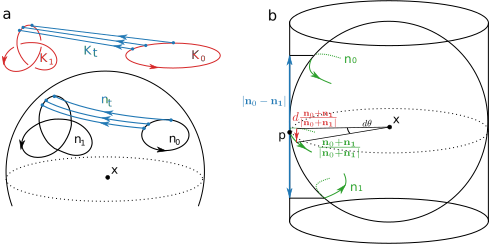
\includegraphics[width = \textwidth]{\MaxwellFigures/Figure12.pdf}
        \caption[Curve homotopy and its projection]{(a) An initial ($K_0$) and final ($K_1$) space curve are connected by a straight line homotopy $K_t$, three lines of which are shown in the figure (blue lines). This projects to a homotopy on the observation sphere via geodesics ${\bf n}_t$ (blue curves) between the initial ${\bf n}_0$ and final ${\bf n}_1$ projected spherical curves. In this figure we deliberately choose $K_0$ and $K_1$ to be different knots --- $K_t$ need not preserve knot type. (b) Calculating the area swept out by the geodesic parameterisation between ${\bf n}_0$ and ${\bf n}_1$. Shown are two segments of ${\bf n}_0$ and ${\bf n}_1$, as well as their normalised average $\frac{{\bf n}_0 + {\bf n}_1}{|{\bf n}_0 + {\bf n}_1|}$ (green curves). Consider the area of the geodesic sliver connecting ${\bf n}_0$ and ${\bf n}_1$ centred on the point ${\bf p}$. Archimedes' theorem tells us this is equal to that same area projected onto a cylinder circumscribing the sphere, which is given by ${|{\bf n}_0 - {\bf n}_1|}d\theta$, or equivalently by the triple product in \eqref{eq:Isotopy}. } 
        \label{fig:Isotopy} 
    \end{figure}

    Consider the contribution to the area of the geodesics connecting a small segment of the two curves, as shown in figure \ref{fig:Isotopy}(b): By Archimedes' theorem on the equality of the area of the sphere and its circumscribed cylinder this is equal to the product of the distance $|{\bf n}_0-{\bf n}_1|$ between the two endpoints of the geodesic arc and the angle swept out by its midpoint $({\bf n}_0+{\bf n}_1)/|{\bf n}_0+{\bf n}_1|$. The difference in solid angle is therefore 
    \begin{align}
        \omega({\bf x}; K_1) - \omega({\bf x}; K_0)
        &=
        \int ({\bf n}_0 - {\bf n}_1) \times \frac{{\bf n}_0 + {\bf n}_1}{|{\bf n}_0 + {\bf n}_1|} \cdot \mathrm{d} \frac{{\bf n}_0 + {\bf n}_1}{|{\bf n}_0 + {\bf n}_1|} \quad  \nonumber \\ 
        &=
        \int \frac{{\bf n}_0 \times {\bf n}_1 \cdot ( \mathrm{d}{\bf n}_0 + \mathrm{d}{\bf n}_1 )}{1+{\bf n}_0 \cdot {\bf n}_1} \quad \textrm{mod } 4\pi.
        \label{eq:Isotopy}
    \end{align}
    This is the basic homotopy formula for solid angle, applicable to an arbitrary deformation of $K$. Both Maxwell's first and third methods of computing $\omega$ can be seen as applications of~\eqref{eq:Isotopy} --- we recover~\eqref{eq:OurSolidAngle1} by letting $K_0$ recede asymptotically far from $\bf x$, so that ${\bf n}_0$ is a single point ${\bf n}_{\infty}$ on the observation sphere and $\omega({\bf x}; K_0)=0$ mod $4\pi$. In \S\ref{sec:GaussBonnet} we shall use a homotopy of $K$ along its tangent developable surface to demonstrate that his second method also follows directly from the homotopy formula. 

    The integral in~\eqref{eq:Isotopy} is not defined when $\bf x$ lies on the surface swept out by $K_t$, which we refer to as the surface of discontinuity --- as an example, in~\eqref{eq:OurSolidAngle1} this surface is formed by translating $K$ to infinity along ${\bf n}_\infty$. The line of $K_t$ passing through $\bf x$ connects antipodal points of the observation sphere, ${\bf n}_0 \cdot {\bf n}_1= -1$, and this line does not project to a unique geodesic arc connecting these endpoints. Instead there is a whole family of equivalent connecting geodesics, which cover the sphere once. As $\bf x$ crosses the surface of discontinuity, the geodesic parameterisation of the antipodal sections of ${\bf n}_0$ and ${\bf n}_1$ jumps from one side of the observation sphere to the other, giving a $4 \pi$ jump in~\eqref{eq:Isotopy}.

    We note that~\eqref{eq:Isotopy} has the same form as the formula given by Fuller for the difference in writhe of two curves~\citep{Fuller1978}. This is because for each fixed point ${\bf x}$ (not on $K_t$ for any $t$) the difference in solid angle is expressible as an area between two spherical curves, as arises for the difference in writhe. This is the first of several relations between the solid angle function for a curve and its writhe, which help to convey its geometric content.

    \section{Maxwell's geometric formula, dual curves and homotopies along tangent developable surfaces }
    \label{sec:GaussBonnet}
    \begin{figure}
        \centering
        \includegraphics{\MaxwellFigures/Figure9.pdf}
        \caption[The dual curve construction.]{A spherical knot projection $\bf n$ (blue curve, here a typical projection of a twisted unknot) induces a dual spherical curve ${\bf n}^* := {\bf t} \times {\bf n}$ (yellow curve). Maxwell proposes the construction of ${\bf n}^*$ by allowing a unit circle (yellow disk) to roll without slipping around $\bf n$ such that its plane of contact is tangent to $\bf n$. A unit vector perpendicular to this circle (yellow arrow) then traces ${\bf n}^*$. As shown in~\eqref{eq:dn*ds}, zeros of geodesic curvature in $\bf n$ correspond to cusps in $\bf n^*$ (marked points). More pictures of this construction may be found in Refs. \citep{Levi1994,Arnold1995}.   }
        \label{fig:DualCurve} 
    \end{figure}
    Maxwell's objection to~\eqref{eq:MaxSphere} is that it involves an arbitrary choice of spherical coordinates on the observation sphere, and for this reason he states a construction in which no such choice is made \citep[Art.~418]{Maxwell2}. Let a unit circle roll without slipping around ${\bf n}$ such that its plane of contact is tangent to $\bf n$, as shown in figure~\ref{fig:DualCurve}(a). Then a unit vector perpendicular to this circle traces a second curve on the observation sphere, called the dual curve ${\bf n}^*$. Denote the length of ${\bf n}^*$ by $\sigma$. Maxwell states that the solid angle is given by 
    \begin{equation}
        \omega({\bf x}) = 2\pi - \sigma ,
        \label{eq:DualCurve}
    \end{equation}
    a result he simply describes as a ``well-known theorem''. This result is in fact equivalent to the Gauss-Bonnet formula~\citep{Lee1996}, an identification that has been rediscovered at least twice~\citep{Levi1994,Arnold1995}. In the form stated by Maxwell,~\eqref{eq:DualCurve} is only correct if ${\bf n}$ is a simple curve without points of inflection, but it is true in much greater generality~\citep{Arnold1995}. As a more general version is essential for application to generic knot projections, we give a self-contained elementary proof, applicable to any smoothly immersed spherical curve. 

    \subsection{A dual curve theorem for self-intersecting curves}
    \label{subsec:GaussBonnetSelfIntersecting}
    \begin{figure}
        \centering
        \includegraphics[width=\textwidth]{\MaxwellFigures/Figure2.pdf}
        \caption[Decomposition of the spherical knot projection.]{The spherical knot projection $\bf n$ in panel (a) may be decomposed via the Seifert algorithm into Seifert circles ${\bf n}_i$, shown in panel (b). These circles bound regions $\Omega_i$, signed according to the orientation of their boundary (coloured hatching). At self-intersection points of $\bf n$, the resulting circles have corners, with exterior angles $\epsilon_{ij}$ (shown for one such corner).}
        \label{fig:GaussBonnet} 
    \end{figure}

    We begin by relating the area swept out by ${\bf n}$ to its integrated geodesic curvature by using the Gauss-Bonnet formula. ${\bf n}$ has a canonical tangent vector induced from the orientation of $K$, denoted $\bf t$, and we choose for it a normal vector $\boldsymbol \gamma := \bf n \times \bf t$, as shown in figure~\ref{fig:Knot}(b). (Note that in the special case that ${\bf n}$ is a simple curve it bounds two regions on the sphere, but is only correctly oriented as the boundary of one of them. ${\boldsymbol \gamma}$ points inwards to this region.) We perform a Seifert decomposition~\citep{Adams2004} of ${\bf n}$. This entails resolving each crossing in a manner that preserves the orientation of the curve and results in its separation into a collection of Seifert circles ${\bf n}_i$, as shown in figure~\ref{fig:GaussBonnet}. Each circle is a simple curve and bounds a region $\Omega_i$. At self-intersections of ${\bf n}$ the Seifert circles have corners, with exterior angles $\epsilon_{ij}$. Now, for each circle, the Gauss-Bonnet formula tells us
    \begin{equation}
        \int_{\Omega_i} \mathrm{d} A  = 2 \pi - \int_{{\bf n}_i} k_{\boldsymbol \gamma} \mathrm{d} s - \sum_j \epsilon_{ij} ,
        \label{eq:GaussBonnetSeifert}
    \end{equation}
    where $k_{\boldsymbol \gamma} = \frac{d {\bf t}}{d s} \cdot {\boldsymbol \gamma}$ is the signed geodesic curvature of the boundary. Summing over all Seifert circles, the left-hand-side gives $\omega({\bf x})$ mod $4\pi$; on the right-hand-side the exterior angles cancel pairwise, and we pick up a contribution of $2\pi S$, where $S$ is the number of Seifert circles, in addition to the total integrated (signed) geodesic curvature. The number of Seifert circles is equal to $\chi + D$, where $\chi$ is the Euler characteristic of the surface constructed by the Seifert algorithm and $D$ is the number of double points (self-intersections)~\citep{Adams2004,Lickorish1997}. For a knot the Euler characteristic of any Seifert surface is odd, so that $S = D+1$ mod $2$. Thus we have
    \begin{equation}
        \omega({\bf x})  = 2 \pi (D + 1) - \int_{{\bf n}} k_{\boldsymbol \gamma} \mathrm{d}s\quad\textrm{mod}\; 4\pi .
        \label{eq:GaussBonnetImmersed}
    \end{equation} 
    We remark that the quantity $D+1$ mod $2$ is the spherical equivalent of the rotation number of a planar self-intersecting curve, sometimes termed its parity \citep{Whitney1937,Phillips1966,Solomon1996}. The $2 \pi$ in the Gauss-Bonnet formula arises as the rotation number of a simple curve, and the appearance of the parity here is thus a natural extension to the self-intersecting case. 

    The integrated geodesic curvature is equal to the (signed) length of the dual curve ${\bf n}^* := -{\boldsymbol \gamma} = {\bf t} \times {\bf n}$ \citep{Levi1994,Arnold1995}(figure~\ref{fig:DualCurve}). To see this, consider how ${\bf n}^*$ varies with arc length along ${\bf n}$:
    \begin{equation}
        \frac{\mathrm{d}{\bf n}^*}{\mathrm{d}s} = \frac{\mathrm{d}\,}{\mathrm{d}s}({\bf t} \times {\bf n}) = \frac{\mathrm{d}{\bf t}}{\mathrm{d}s} \times {\bf n}= k_{{\boldsymbol \gamma}} {\bf t} .
        \label{eq:dn*ds}
    \end{equation}
    ${\bf t}$ is tangent to ${\bf n}^*$, but its orientation alternates across zeros of $k_{\boldsymbol \gamma}$, which correspond to cusps in ${\bf n}^*$. Defining $ds^* = k_{\boldsymbol \gamma}ds$, we obtain $\mathrm{d}{\bf n}^*/\mathrm{d}s^* = {\bf t}$, and see that $ds^*$ should be interpreted as a signed length element, the sign being given by that of $k_{\boldsymbol \gamma}$. Thus we arrive at
    \begin{equation}
        \omega({\bf x}) =  2 \pi (D+1) - \int_{{\bf n}^*} \mathrm{d} s^* \quad \mathrm{mod}\; 4\pi . 
        \label{eq:DualCurveImmersed}
    \end{equation}
    For a simple curve without inflection points $D=0$ and the sign of $\mathrm{d}s^*$ never alternates, so its integral gives $\sigma$ and we recover~\eqref{eq:DualCurve}. By contrast, consider the spherical `figure-eight' curve $\bf {n}$ shown in figure~\ref{fig:DualCurve}, as would arise when $K$ is a twisted unknot parameterised by $(\sin t, \cos t, \sin 2t), t\in [0,2\pi]$, and the point of projection lies on the $y$-axis with $|y|>1$. Considering a surface spanning this twisted unknot, one immeadiately expects $\omega=0$ at such a projection point --- let us check the results of \eqref{eq:DualCurve}, \eqref{eq:DualCurveImmersed} applied to the spherical figure-eight curve. $D=1$ and we have two zeros of geodesic curvature, which divide $\bf{n}^*$ into two segments separated by cusps with $ds^*$ switching sign between them. So applying~\eqref{eq:DualCurveImmersed}, we arrive at our expected result, but applying~\eqref{eq:DualCurve} we do not. Eq.~\eqref{eq:DualCurveImmersed} thus generalises Maxwell's ``well known theorem''~\eqref{eq:DualCurve} to the case of a smoothly immersed curve, and in particular to any generic spherical knot projection. 

    \subsection{The pullback to $K$ and a homotopy along the tangent developable surface}
    \label{subsec:Pullback}

    As a result on the structure of spherical areas,~\eqref{eq:DualCurveImmersed} is valid for any smoothly immersed spherical curve. However, we have in mind the case where one arises as the projection of the knot $K$. Using this projection we now pull each term in~\eqref{eq:DualCurveImmersed} back to $K$. This facilitates a reinterpretation in terms of the geometry of $K$, as well as a novel method of deriving it using~\eqref{eq:Isotopy}.

    We begin by constructing a natural `projective' framing for $K$, dependent on $\bf x$, with which we will express $D$ in~\eqref{eq:DualCurveImmersed} as a self-linking number. To construct this framing, extend the lines of sight from ${\bf x}$ along ${\bf n}$ until they meet $K$. These lines project to vectors normal to $K$, which are non-zero provided ${\bf n} \cdot {\bf T} \neq \pm 1$ where ${\bf T}$ is the unit tangent vector to $K$, in other words provided there are no cusps in ${\bf n}$ on the observation sphere. The number of double points seen from $\bf x$ mod $2$ is equal to the self-linking number of $K$ given this projective framing, $\mathrm{SL}(K,{\bf x})$, also mod $2$. The mod $2$ counting gives an ambiguity in the sign of the identification of $D$ with $\mathrm{SL}(K,{\bf x})$ which will lead to two distinct re-writings of~\eqref{eq:DualCurveImmersed}, and so we shall keep the sign explicit in the following. 

    Using C\u{a}lug\u{a}reanu's theorem~\citep{Calugareanu1959,Calugareanu1961}, $ \mathrm{SL}(K,{\bf x}) = \mathrm{Tw}(K,{\bf x}) +\mathrm{Wr}(K)$, we now write $ \mathrm{SL}(K,{\bf x})$ in terms of the writhe of $K$ and the twist of the projective framing, which is directly computed to be 
    \begin{equation}
        \mathrm{Tw}(K,{\bf x}) = \int_K  \frac{ ( {\bf n} \cdot {\bf T} ) ({\bf n} \cdot {\bf T} \times \mathrm{d}{\bf T}) }{1 - ({\bf n} \cdot {\bf T})^2} . 
        \label{eq:Twist}
    \end{equation}
    Substituting this expression for $\mathrm{SL}(K,{\bf x})$ into~\eqref{eq:DualCurveImmersed} with the sign ambiguity discussed above, and combining with the pullback of the dual curve length,
    \begin{equation}
        \int_{{\bf n ^*}} \mathrm{d} s^* = \int_{{\bf n}} k_{\bf \boldsymbol \gamma } \mathrm{d} s = \int_K  \frac{ {\bf n} \cdot {\bf T} \times \mathrm{d}{\bf T} }{1 - ({\bf n} \cdot {\bf T})^2},
        \label{eq:geodesicpullback1}
    \end{equation}
    we arrive at
    \begin{equation}
        \omega({\bf x}) = 2 \pi(1 \pm \mathrm{Wr}(K)) - \int_K  \frac{ {\bf n} \cdot {\bf T} \times \mathrm{d}{\bf T} }{1 \pm {\bf n} \cdot {\bf T}}  \quad \mathrm{mod}\; 4\pi .
        \label{eq:OurSolidAngle2}
    \end{equation}    
    \begin{figure}[t]
        \begin{centering}
            \includegraphics[ width = 0.4\textwidth ]{\MaxwellFigures/Figure5.pdf}
            \caption[Homotopy along the tangent developable surface.]{The forward tangent developable surface ${\bf{T}}_{t,+}$ (yellow surface) for the knot $K$ in figure~\ref{fig:Knot} (red curve), constructed by extending half-lines along tangents from $K$ (green, dashed). The intersection of the surface with a sphere of asymptotically large radius gives a scaled copy of the tangent indicatrix to $K$, ${\bf T}_{\infty,+}$ (blue). The half-lines comprising ${\bf T}_{t,+}$ define a straight line homotopy between $K$ and ${\bf T}_{\infty,+}$, from which the blue, dashed curve is taken.}
            \label{fig:TangentDevelopable}
        \end{centering}
    \end{figure}
    This formula for the solid angle depends only on $K$ and data canonically associated to it, with the only ambiguity being a choice of sign. The appearance of the writhe in~\eqref{eq:OurSolidAngle2} reveals this geometric property of curves to be closely connected to the solid angle. We shall return to the sign ambiguity in a moment --- for now, let us select the plus sign. 

    Instead of taking~\eqref{eq:DualCurve} as our starting point, we now demonstrate how~\eqref{eq:OurSolidAngle2} may be derived directly from the curve homotopy formula~\eqref{eq:Isotopy}. To construct the appropriate homotopy, extend half-lines from $K$ along its tangents ${\bf T}$, sweeping out a surface in space known as the forward tangent developable surface of $K$, which we denote ${\bf{T}}_{t,+}:={\bf y} + t {\bf T}$, $t\in [0,\infty)$~\citep{Eisenhart} --- an example of this surface is shown in figure~\ref{fig:TangentDevelopable}. Consider the intersection of this surface with a sphere of asymptotically large radius. The curve ${\bf T}_{\infty, +}$ given by this intersection is simply the spherical image of $\bf T$, known as the forward tangent indicatrix of $K$ ~\citep{Eisenhart}, scaled to the sphere radius. Our desired homotopy is between $\bf T_{\infty,+}$ and $K$, and is defined by the half-lines comprising ${\bf{T}}_{t,+}$. As $\bf T_{\infty,+}$ is asymptotically far from ${\bf x}$, its projection on to the observation sphere simply reproduces the tangent indicatrix. Using the fact that ${\bf n} \times {\bf T} \cdot \mathrm{d}{\bf n} = 0$, we see that the integral in~\eqref{eq:OurSolidAngle2} is a second special case of~\eqref{eq:Isotopy}, with $K_0 = {\bf T}_{\infty,+}$, $K_1 =K$, and the area swept out on the observation sphere lying between the forward tangent indicatrix and $\bf n$. 

    This argument also identifies $2\pi(1+\mathrm{Wr}(K))$ as the solid angle of $\bf T_{\infty,+}$. We may obtain an integral formula for this area by considering the asymptotics of~\eqref{eq:OurSolidAngle2}, allowing ${\bf x}$ to recede far from $K$ along $-{\bf n}_{\infty}$ so that $\omega({\bf x}) \rightarrow 0$. Doing so yields
    \begin{equation}
        \int_K  \frac{ {\bf n}_\infty \cdot {\bf T} \times \mathrm{d}{\bf T} }{1 + {\bf n}_\infty \cdot {\bf T}} = 2 \pi(1 + \mathrm{Wr}(K))  \quad \textrm{mod}\; 4\pi , 
        \label{eq:AsymptoticSolidAngle2}
    \end{equation}
    however, as this integral is the area bound by the tangent indicatrix on the unit sphere, the identification is simply a recovery of Fuller's writhe mod $2$ formula~\citep{Fuller1978}. In the context of curve homotopies, we may interpret~\eqref{eq:AsymptoticSolidAngle2} as giving the change in solid angle for a homotopy in which $\bf T_{\infty,+}$ shrinks to a point (that projects to ${\bf n}_\infty$ on the observation sphere). Eq.~\eqref{eq:OurSolidAngle2} may then be thought of as a combination of two homotopies: the first from an arbitrary point to $\bf T_{\infty,+}$, and the second from $\bf T_{\infty,+}$ to $K$. By contrast,~\eqref{eq:OurSolidAngle1} combines these two homotopies into one. Returning to the sign choice made above, we now see that choosing a minus sign would give a version of~\eqref{eq:OurSolidAngle2} corresponding to a homotopy along the backward tangent developable surface ${\bf{T}}_{t,-}:={\bf y} - t {\bf T}$, $t\in [0,\infty)$, between $K$ and the backward tangent indicatrix $\bf T_{\infty,-}$. That aside, the geometric interpretation remains the same. We note briefly that the tangent indicatrix is not the only spherical curve canonically associated with $K$ which might be used to define a homotopy; we might also consider the normal and binormal indicatrices. In these cases, however, neither triple product in~\eqref{eq:Isotopy} vanishes, as occurred in~\eqref{eq:OurSolidAngle2}, and so the resulting formulae are less simple. 

    With the choice of plus (minus) sign in~\eqref{eq:OurSolidAngle2}, the surface of discontinuity discussed in \S\ref{sec:CurveIsotopies} is given by ${\bf T}_{t,+}$ (${\bf T}_{t,-}$). Jumps are also present in~\eqref{eq:GaussBonnetImmersed} and~\eqref{eq:DualCurveImmersed}, however they occur on both halves of the tangent developable surface ${\bf T}_{t,+}\cup {\bf T}_{t,-}$ and the overall $4 \pi$ jumps are composed of each individual term in the equations jumping by $2 \pi$. To convince ourselves of this fact, consider the behaviour of~\eqref{eq:DualCurveImmersed} as ${\bf x}$ passes across ${\bf T}_{t,+}\cup {\bf T}_{t,-}$. ${\bf n}$ undergoes a Reidemeister 1 move, during which $D$ jumps by 1. The segment of ${\bf n}^*$ corresponding to the Reidemeister move in ${\bf n}$ begins and ends at antipodal points on the sphere. By removing the loop in ${\bf n}$, we create two inflection points. Recalling that the sign of $ds^*$ alternates between these inflections, we pick up a change in signed length of $2 \pi$.


    \section{The structure of $\omega$}
    \label{sec:LocalStructure}

    The level sets of $\omega$, for regular values, form a family of Seifert surfaces with common boundary $K$. Figure~\ref{fig:SolidAngle} shows this global structure for a twisted unknot and a Whitehead link. 
    The topology of the level sets changes at critical points of $\omega$, where generically the local structure is a cone point $\pm(x^2+y^2-2z^2)$ with Morse index $1$ or $2$. As the solid angle is a harmonic function, critical points of Morse index $0$ or $3$ are forbidden by the maximum principle. For knots and links that are fibred~\citep{Stallings1978} it is possible for the solid angle to have no critical points at all; indeed this is the case for both the unknot and Whitehead link shown in figure~\ref{fig:SolidAngle}. The general relationship between the shape and geometry of a knot or link and critical points of the solid angle is a fascinating open problem. 

    It is of particular interest to characterise $\omega$ in a tubular neighbourhood of $K$, so that we may modify it when initialising simulations using $\omega$. This control is useful when the local structure of the field around a vortex affects its dynamics, as for example in helicity in fluids~\citep{Moffat1992} or the twist of scroll waves in the FitzHugh-Nagumo model~\citep{Winfree1984,Maucher2018}. This local structure has longitudinal and transverse parts: the level sets of $\omega$ rotate as one traverses $K$, and in a plane normal to $K$ corrections due to local curvature and torsion arise, analogous to those studied for the magnetic field about a curved wire~\citep{Saffman1992}. Harmonic fields in the tubular neighbourhood of a knot have also recently been studied in Ref.~\citep{Duan2018}. 

    \begin{figure}[htbp]
        \begin{centering}
            \includegraphics[clip = true, trim = 120 380 120 0, width = 0.9\textwidth ]{\MaxwellFigures/Figure3.pdf}
            \caption[The structure of solid angle around a knotted curve.]{The structure of $\omega$ around a knotted curve, generated with the method of \S\ref{sec:NumericalImplementation}. (a)--(c) show level sets of $\omega$ of spacing $\frac{\pi}{2}$, each of which forms a Seifert Surface for the knot with opacities on the near sides of the images reduced to reveal the inner structure of $\omega$. (a) A twisted unknot. (b,)~(c) The Whitehead link (components in blue, green) from two viewing directions. (d) A slice through the Whitehead link from the same direction as (c). The local structure of $\omega$ about the knot is especially clear in (d) --- $\omega$ winds by $4 \pi$, and as we move away from the knot, curvature induced corrections cause the level sets of $\omega$ to bunch along the curve normal, as discussed in \S\ref{sec:LocalStructure}.}
            \label{fig:SolidAngle}
        \end{centering}
    \end{figure}

    \subsection{Longitudinal structure --- the solid angle framing}
    \begin{figure}[t]
        \makebox[0.9\textwidth][c]{\includegraphics[clip = true, trim = 0 580 0 0, width= \paperwidth ]{\MaxwellFigures/Figure4.pdf}}
        \caption[The solid angle framing.]{(a) The solid angle framing for the Whitehead link of figure~\ref{fig:SolidAngle}. Shown is the level set $\omega =0$ (blue surface), and its induced framing (components in blue, green). (b) The limiting behaviour of $\bf n$ as $\bf x$ approaches $K$ (shown is the behaviour of $\bf n$ about the marked point on the $4_1$ of figure~\ref{fig:Knot}). $\bf x$ approaches a fixed point ${\bf y}(s)$ on $K$ such that ${\bf u} := {\bf x} - {\bf y}(s) = (\epsilon \cos\theta, \epsilon \sin\theta,0)$ lies in the normal plane to ${\bf y} (s)$. As $\epsilon/\rho \rightarrow 0$, a region on $K$ of size $\sqrt{ 2 \rho \epsilon}$ (green) projects to a semicircle $\mathcal{S}_{s,\theta}$ between $\pm{\bf T}(s)$. This semicircle sweeps the observation sphere as $\theta$ is varied. The remainder of $K$ projects to $\mathcal{C}_s$ (red), and is independent of $\theta$.} 
        \label{fig:LocalStructure}
    \end{figure}

    The intersection of the level set $\omega=0$ with $K$ defines a `solid angle' framing, canonical in the sense that it depends only on the knot and is purely geometric. As this framing is described by a pushoff of $K$ onto an orientable surface, it has zero self-linking number~\citep{Lickorish1997}; the extension to links is straightforward and discussed in \S~\ref{sec:NumericalImplementation}. Figure~\ref{fig:LocalStructure}(a) shows this surface and its induced framing for the Whitehead link of figure~\ref{fig:SolidAngle}. A natural question is to identify this solid angle framing in terms of the curve geometry. Let ${\bf x}$ approach a particular point ${\bf y}(s) \in K$, for a fixed $s$, in such a way that the displacement vector ${\bf u} := {\bf x} - {\bf y}(s)$ defines a direction in the normal plane to the curve at $s$ (figure~\ref{fig:LocalStructure}(b)). Aligning the $x,y,z$ axes with the local Frenet-Serret frame ${\bf N}(s),{\bf B}(s),{\bf T}(s)$, we have ${\bf u} = (\epsilon \cos\theta, \epsilon \sin\theta,0)$. As $\epsilon/\rho \rightarrow 0$, where $\rho$ is the radius of curvature, we may think of the image of $K$ on the observation sphere as comprised of two parts; for points ${\bf y}(s')$ with $s'$ outside a small interval $I$ around $s$ (of size $\sim\sqrt{2\rho \epsilon}$), the projection to ${\bf x}$ is no different from the projection to ${\bf y}(s)$, and the image of $K$ is given by the unit chords $\frac{{\bf y}(s') - {\bf y}(s)}{|{\bf y}(s') - {\bf y}(s)|}$. This is a curve $\mathcal{C}_s$ on the observation sphere with endpoints $\pm {\bf T}(s)$ and is independent of $\theta$. In the same limit, the points ${\bf y}(s^{\prime})$ with $s^{\prime}\in I$ contribute to the image of $K$ on the observation sphere a semicircle $\mathcal{S}_{s,\theta}$ between $\pm{\bf T}(s)$ with midpoint $- \frac{{\bf u}}{|{\bf u}|}$ that depends on $\theta$. ${\bf n}$ is thus decomposed as ${\bf n} = \mathcal{C}_s \cup \mathcal{S}_{s,\theta}$. Varying $\theta$, $\mathcal{C}_s$ remains unchanged, and $\mathcal{S}_{s,\theta}$ wraps the sphere once, giving the asymptotic winding structure $\omega = 2(\theta - \alpha(s))$, where $\alpha(s)$ is the rotation angle of the Frenet-Serret normal ${\bf N}(s)$ into the solid angle framing. $\alpha(s)$ gives the longitudinal structure of $\omega$. It represents the contribution of $\mathcal{C}_s$ to $\omega$, and as such is a global quantity, not computable by a local analysis. 

    Our decomposition of ${\bf n}$ is identical to that of the set of cross chords considered in the context of C\u{a}lug\u{a}reanu's theorem~\citep{Dennis2005,Calugareanu1959}, a consequence of the projection map outside of $I$ degenerating to the chord map as $\epsilon/\rho \rightarrow 0$ to give $\mathcal{C}_s$. The completion of $\mathcal{C}_s$ by $\mathcal{S}_{s,\theta}$ is given, in C\u{a}lug\u{a}reanu's theorem, by a choice of framing vector ${\bf u}$ for $K$~\citep{Dennis2005}. Here it is given, via projection, by the displacement vector ${\bf u}$.

    As discussed by Dennis \& Hannay in Ref.~\citep{Dennis2005}, given some framing ${\bf u}$, $\mathrm{Wr}(K)$ and $\mathrm{Tw}(K, {\bf u})$ are given by the areas swept out on an abstract sphere by $\mathcal{C}_s$ and $\mathcal{S}_{s,\theta}$ respectively, as $s$ varies along $K$. They point out that one may choose a special framing, which they call the `writhe framing', such that the area swept out by $\mathcal{S}_{s,\theta}$ precisely cancels that swept out by $\mathcal{C}_s$, giving zero self-linking number. The discussion above makes clear this framing is exactly the solid angle framing, and the cancellation condition may be naturally read as a variation of $\theta$ such that $\frac{{\bf u}}{|{\bf u}|}$ lies tangent to the level set $\omega = 0$; in terms of the Frenet-Serret frame, $\theta= \alpha(s)$.

    \subsection{Transverse structure --- curvature induced corrections to $\omega$}

    In the previous section, we saw that the asymptotic structure of $\omega$ normal to $K$, corresponding to the decomposition ${\bf n} = \mathcal{C}_s \cup \mathcal{S}_{s,\theta}$, is simply $\omega = 2( \theta - \alpha(s))$. At finite $\epsilon/\rho$ we find corrections due to the local curvature of $K$, with the leading contribution being logarithmic in $\epsilon$. For the derivative of $\omega$, the magnetic field, this problem is well studied \citep{Saffman1992,Ricca1994}. However, we wish to demonstrate that existing results may be mapped directly on to corrections in the geometry of $\bf n$ as the decomposition ${\bf n} = \mathcal{C}_s \cup \mathcal{S}_{s,\theta}$ is smoothed at finite $\epsilon/\rho$, insight one does not gain from the magnetostatic picture.

    The asymptotic description ${\bf n} = \mathcal{C}_s \cup \mathcal{S}_{s,\theta}$ contains cusps at the boundary between $\mathcal{C}_s$ and $\mathcal{S}_{s,\theta}$, located at $\pm {\bf T}(s)$. The primary effect of small but finite $\epsilon/\rho$ is a rounding of these cusps, and the displacement of ${\bf n}$ slightly off $\pm {\bf T}(s)$, as shown in figure~\ref{fig:CurvatureCorrections}(a). It is thus natural to focus our attention, and chose coordinates, appropriate to describing $\bf n$ in the vicinity of $\pm {\bf T}(s)$. Expanding ${\bf y}(s')$ to lowest order in $s'$, ${\bf y}(s') = (\frac{1}{2\rho}(s'-s)^2,0,s'-s)$ and $\bf n$ is given by
    \begin{equation}
        {\bf n} = \biggl[1 + \frac{\tilde{\epsilon}}{2} \biggr(\tilde{s}^2 +\frac{1}{\tilde{s}^2}\biggl)- \tilde{\epsilon}\cos \theta \biggr]^{-\frac{1}{2}} 
        \biggr(
        \sqrt{\frac{\tilde{\epsilon}}{2}}\frac{1}{\tilde{s}} (\tilde{s}^2 - \cos \theta),
        -\sqrt{\frac{\tilde{\epsilon}}{2}}\frac{1}{\tilde{s}} \sin \theta,
        1
        \biggl),
        \label{eq:FirstCurvatureCorrectedn}
    \end{equation}
    where we have defined reduced lengthscales $\tilde{\epsilon}:=\frac{\epsilon}{\rho}$, $\tilde{s} :=\frac{s'-s}{\sqrt{2\epsilon \rho}}$. The form of~\eqref{eq:FirstCurvatureCorrectedn} is chosen to emphasise that we have an expansion of $\bf n$ in the vicinity of $\pm{\bf T}(s)$ on the observation sphere. Focusing now on the smoothed cusp at positive $\tilde{s}$, we introduce a new variable $t :=\ln(\tilde{s})$, and rotate the $x$-$y$ coordinates of ${\bf n}$ by $\frac{\theta}{2}$, yielding 
    \begin{equation}
        {\bf n}
        = [1 + \tilde{\epsilon}(\cosh 2t - \cos \theta )]^{-\frac{1}{2}}
        \biggr(
        \sqrt{2\tilde{\epsilon}} \cos \frac{\theta}{2} \sinh t, 
        -\sqrt{2\tilde{\epsilon}}\sin \frac{\theta}{2} \cosh t,
        1
        \biggl),
        \label{eq:CurvatureCorrectedn}
    \end{equation}
    a hyperbola projected onto the observation sphere (figure~\ref{fig:CurvatureCorrections}(a)). In the original, unrotated coordinates, the asymptotic behaviour of this hyperbola is of two longitudinal great circles passing through ${\bf T}(s)$ at angles $\theta$ and $0$. As $\tilde{\epsilon}\rightarrow 0$, the first of these circles gives $\mathcal{S}_{s,\theta}$. The second gives the local structure of $\mathcal{C}_s $, and in particular tells us that the direction of departure of $\mathcal{C}_s$ from ${\bf T}(s)$ is set by ${\bf N}(s)$. The vertex of the hyperbola, found at $t = 0$, is the point of closest approach to ${\bf T}(s)$ and gives the natural choice $\tilde{s} =1$ ($s' = s + \sqrt{2\rho \epsilon}$) to define the upper boundary between $\mathcal{S}_{s,\theta}$ and $\mathcal{C}_s $. It approaches the pole as $\sqrt{{\tilde{\epsilon}}}$, and so in the limit $\tilde{\epsilon} \rightarrow 0$ we recover the sharp decomposition ${\bf n} = \mathcal{C}_s \cup \mathcal{S}_{s,\theta}$.

    The local structure of the solid angle can be computed using any of our formulae for $\omega$, however, in view of the foregoing description, an appealing method is to use~\eqref{eq:GaussBonnetImmersed} and the geodesic curvature of the hyperbola. As this approach is symmetric in $\tilde{s}$, it is enough to compute the geodesic curvature for the hyperbola near $\tilde{s}=1$ and simply double the result to account for $\tilde{s}=-1$. Further, the geodesic curvature of $\bf n$ is strongly peaked in a localised region of size $\sim\sqrt{\tilde{\epsilon}}$ about the vertex of the hyperbola, decaying to $0$ as the hyperbola approaches its asymptotic great circles. 
    Using~\eqref{eq:CurvatureCorrectedn} we find an integrated geodesic curvature of 
    \begin{equation}
        -2 \int_{-\infty}^{\infty}\frac{\sin \theta\sqrt{1+\tilde{\epsilon}( \cosh 2t - \cos \theta)} }{\cos \theta + \cosh 2t + \tilde{\epsilon} \sin^2 \theta } \mathrm{d}t,
        \label{eq:CurvatureCorrectionIntegration}
    \end{equation} 
    where we have extended the upper limit of integration to $+\infty$, corresponding to an integration of the hyperbola between $- \frac{{\bf u}}{|{\bf u}|}$ and ${\bf N}(s)$ on the observation sphere. The integrand decays exponentially for large $t$ so that the error involved is small. 

    The integral~\eqref{eq:CurvatureCorrectionIntegration} may be evaluated exactly in terms of elliptic integrals of the first and third kind. The main feature is that the result is not analytic in $\tilde{\epsilon}$ but has leading behaviour $\tilde{\epsilon} \ln \tilde{\epsilon}$. This can be seen most easily by noting that the integrand decays exponentially for $|t| \gtrsim \frac{1}{2} \ln (2/\tilde{\epsilon})$ and that the integral is dominated by values of $|t|$ smaller than this. 
    Retaining only the leading behaviour, one finds the local structure of the solid angle has the form 
    \begin{equation}
        \omega(\tilde{\epsilon}, \theta)= 2 \bigl( \theta-\alpha(s) \bigr) + \tilde{\epsilon} \ln \frac{8}{\tilde{\epsilon}}\, \sin \theta + O(\tilde{\epsilon}) ,
        \label{eq:CurvatureCorrection}
    \end{equation} 
    in which a zeroth order term from the integrated geodesic curvature gives the winding of $\omega$ and the logarithmic term causes the level sets of $\omega$ to bunch along the local normal. Figure~\ref{fig:SolidAngle}(d) shows a cross-section through a Whitehead link in which both of these structures are clearly visible. In figure~\ref{fig:CurvatureCorrections}(b) we compare the various orders of approximation in~\eqref{eq:CurvatureCorrection} to the exact solution for a round unknot. In contrast to the divergence of the magnetic field, $\omega$ is perfectly well behaved as $\tilde{\epsilon} \rightarrow 0$. The logarithmic correction $\tilde{\epsilon} \log \tilde{\epsilon}$ tends to $0$, but in a cusped manner, with unbounded radial derivative at the origin. We may interpret this fact as a direct consequence of the limiting cusped structure ${\bf n} = \mathcal{C}_s \cup \mathcal{S}_{s,\theta}$ --- the magnetic field gives the rate of change in the area of a spherical curve as we smooth a cusp in it, and is thus naturally unbounded. 

    We note briefly that~\eqref{eq:CurvatureCorrection} is not harmonic --- indeed, the corresponding expression for the magnetic field found in, for example, \citep{Saffman1992} is not divergence free. This is a consequence of neglecting variation in $\omega$ along ${\bf T} (s)$ and one may verify that, allowing $\bf {x}$ to lie off the plane normal to ${\bf y}(s)$, one picks up a term linear in $z$ which restores harmonicity. 

    \begin{figure}[htbp]
        \begin{centering}
            \includegraphics[clip = true, trim = 120 580 120 0, width = 0.9\textwidth ]{\MaxwellFigures/Figure6.pdf}
            \caption[Transverse solid angle structure.]{(a) For finite $\epsilon/\rho$, the local structure of $\bf n$ is approximated by the hyperbola~\eqref{eq:CurvatureCorrectedn} --- the dashed black line gives the approximation to $\bf n$ shown in figure~\ref{fig:LocalStructure}. As $\epsilon /\rho \rightarrow 0$, the vertex of this hyperbola approaches ${\bf T}(s)$, and the asymptotes remain unchanged (black dotted line). In this way, we obtain the limiting decomposition ${\bf n} = \mathcal{C}_s \cup \mathcal{S}_{s,\theta}$. The two asymptotes are great circles through ${\bf T}(s)$ at angles $\theta$ and $0$, and give the local behaviour of $\mathcal{S}_{s,\theta}$ and $\mathcal{C}_s$ --- note that that an angle of $0$ corresponds to the direction ${\bf N}(s)$. (b) The local structure of $\omega$ in a plane normal to $K$. Contours of spacing $\frac{\pi}{3}$ are shown for the the zeroth order rotational structure (black dashed line), the curvature induced correction~\eqref{eq:CurvatureCorrection} (green) and the exact solution for a circle of radius $\rho$ (blue). The absolute values of the level sets are arbitrary, as we have discarded global information about $\mathcal{C}_s$ in our local structure calculations. The primary effect of curvature is to bunch the level sets of $\omega$ along the local normal. Note that for the curvature induced correction we have fixed the regular values in~\eqref{eq:CurvatureCorrection} to zero by comparison with the exact solution for a circle \citep{Saffman1992}.}
            \label{fig:CurvatureCorrections}
        \end{centering}
    \end{figure}

    \section{Remarks on numerical implementation, extension to links}
    \label{sec:NumericalImplementation}

    In~\eqref{eq:OurSolidAngle1},~\eqref{eq:GaussBonnetImmersed},~\eqref{eq:DualCurveImmersed} and~\eqref{eq:OurSolidAngle2}, we have several possible methods for computing $\omega$ for any curve $K$, directly from the specification of its embedding in $\mathbb{R}^3$. The main difficulties in their numerical implementation are encountered when evaluating $\omega(\bf x)$ at points close to the surface of discontinuity discussed in \S\ref{sec:CurveIsotopies}, \ref{subsec:Pullback}. We shall focus discussion on~\eqref{eq:OurSolidAngle1} and~\eqref{eq:OurSolidAngle2}, the remaining equations being of similar numerical character.

    Focusing first upon~\eqref{eq:OurSolidAngle1}, when $\bf x$ lies on the surface of discontinuity it is pierced by a (generically) unique half-line extended from some point ${\bf y}(s) \in K$ such that ${\bf n}(s) \cdot {\bf n}_\infty = -1$. Considering the integral in~\eqref{eq:OurSolidAngle1} to be defined upon $K$, at the arc length $s$ there is an isolated point of divergence in the integrand. In the degenerate case where ${\bf x}$ lies upon a line of self-intersection in the surface, there will be multiple such points. Letting ${\bf x}$ now lie slightly off the surface and approach it perpendicularly, we may expand the integrand of~\eqref{eq:OurSolidAngle1} using ${\bf x}-{\bf y}(s) := \epsilon \cos \theta\, {\bf n}_\infty + \epsilon \sin \theta\, {\bf n}_\infty \times {\bf T}(s) / |{\bf n}_\infty \times {\bf T}(s)| $, where $\theta$ is now the angle between $ {\bf x}-{\bf y}(s)$ and the surface. We find that its limiting behaviour is that of a Lorentzian peak of width $\epsilon \theta$, which abruptly switches sign as ${\bf x}$ crosses the surface. If one employs a simple numerical integration scheme with regularly spaced points along $K$ of spacing $\Delta s$, the Lorentzian peak is not captured when $\epsilon \theta \approx \Delta s$. This leads to poor approximation of $\omega({\bf x})$ in a region of constant thickness $\Delta s$ about the surface of discontinuity. By refining $K$, we may reduce the thickness of this region --- unsurprisingly, this result suggests that $\Delta s$ should be on the order of the resolution one desires for $\omega$.

    A similar discussion holds for~\eqref{eq:OurSolidAngle2}, for which the divergences of the integrand occur at $s$ such that ${\bf n}(s)\cdot{\bf T}(s) = \pm 1$, depending on which homotopy is used. The width of the Lorentzian peak instead scales as $\rho(s) \theta$, and so the thickness of the region of poor approximation is $\Delta s \epsilon/ \rho (s)$; in particular, we note that this thickness scales with viewing distance in~\eqref{eq:OurSolidAngle2}, but not in~\eqref{eq:OurSolidAngle1}.

    One method of avoiding these peaks is to use the freedom in~\eqref{eq:OurSolidAngle1},~\eqref{eq:OurSolidAngle2} to move the surface of discontinuity about in space, ensuring ${\bf x}$ is never too close to it when computing $\omega({\bf x})$. In~\eqref{eq:OurSolidAngle1}, we have freedom in our choice of ${\bf n}_\infty$. The surface of discontinuity is given by dragging $K$ to infinity along ${\bf n}_\infty$, and two different choices of ${\bf n}_\infty$ will give two such surfaces. If $K$ is knotted, these surfaces must intersect, giving a set of curves on which a third choice of ${\bf n}_\infty$ is needed. In practice, an initial choice of ${\bf n}_\infty$ is often suggested by the geometry of the input knot, or is simply chosen to be a coordinate axis. When computing $\omega({\bf x})$, one may record the minimum value of ${\bf n}\cdot {\bf n}_\infty$ and, if it crosses some user defined threshold, switch to using $-{\bf n}_\infty$ for the calculation at that point. On the set of lines where this second choice again crosses the threshold, a random choice of ${\bf n}_\infty$ may be used.~\eqref{eq:OurSolidAngle2} faces analogous problems on the tangent developable surface. Here, we have freedom in whether to place the discontinuity on ${\bf T}_{t,+}$ or ${\bf T}_{t,-}$. However, these two surfaces again generically intersect \citep{Cleave1980,Mond1989}, and there is now no more freedom in $\eqref{eq:OurSolidAngle2}$, forcing one to either switch method or analytically correct for the Lorentzian peaks along such intersections. For this reason, and for the scaling properties discussed above, from a numerical standpoint we have found the use of~\eqref{eq:OurSolidAngle1} to be more convenient than~\eqref{eq:OurSolidAngle2}. 

    Two brief computational remarks: As discussed in \S\ref{sec:LocalStructure}, the limiting local structure of $\omega$ about $K$ has cylindrical symmetry. If one desires high accuracy to sample the tubular neighbourhood of $K$, one may use a cylindrical mesh out to a distance ${\sim}\rho(s)$. Finally, we note that as values of $\omega$ for different values of $\bf x$ are computed independently of one another, our formulae are easily parallelised. 

    \subsection{Extension to links}
    Extending our results to links is straightforward: by the linearity of electromagnetism, one simply sums $\omega$ mod $4 \pi$ for each component of $K$. We reiterate that $\omega$ is only defined for oriented curves, and that different choices of orientation for each component of $K$ will give distinct solid angle functions. In the case of the solid angle framing discussed in \S\ref{sec:LocalStructure}, each component $K_i$ acquires a framing, whose self-linking number equals the negative of the sum of the linking numbers between $K_i$ and $K_j$, $j \neq i$ (figure~\ref{fig:LocalStructure}).

    \section{Construction of knotted fields: two illustrations}

    We describe briefly two different examples of knotted fields that can be constructed using the solid angle as illustrations of how it influences the structure in different settings. 

    \subsection{Scroll waves in excitable media}
    \label{subsec:scroll}

    The possibility of knotting in the waves of excitable media has been considered for some time~\citep{Winfree1983,Winfree1984}. In a three-dimensional excitable medium, scroll waves of excitation emanate from a vortex filament, which it is possible to close into a loop or knot. Recent results have highlighted a remarkable topology-preserving dynamics in these materials~\citep{Maucher2016,Maucher2017,Maucher2018} in which the geometric shape of the vortex filament relaxes and simplifies but without strand crossings, thus preserving the topology. Simple effective curve dynamics seem insufficient to capture the full behaviour, which depends also on interactions mediated by the global structure of the scroll waves. This structure can be captured, in part at least, using the solid angle. 

    \begin{figure}[htbp]
        \centering
        \includegraphics[width=.5\textwidth]{\MaxwellFigures/Figure7}
        \caption[Constructing scroll waves from solid angle.]{Scroll waves from a unknotted vortex filament. In (a) we show the zero level set of the phase field~\eqref{eq:scroll} and in (b) a modification of it where a sinusoidal modulation has been added to the solid angle framing, thereby adjusting the local spin rate of the scroll wave. In both (a) and (b) the two columns simply show different cuts through the emanating scroll waves.}
        \label{fig:scroll}
    \end{figure}

    Scroll waves emanate from a knotted vortex filament creating an outward propagating family of approximately equi-spaced wavefronts. A simplified description of this wave system is given by a phase field that both winds by $2\pi$ around the filament curve and increases linearly with distance from it. This behaviour is captured by the function 
    \begin{equation}
        \psi({\bf x}) = k d_{K}({\bf x}) + \frac{1}{2} \omega_{K}({\bf x}) \quad \textrm{mod}\; 2\pi ,
        \label{eq:scroll}
    \end{equation} 
    where $\omega_K({\bf x})$ is the solid angle of $K$, $d_{K}({\bf x}) = \min_{{\bf y} \in K} |{\bf y}-{\bf x}|$ is the distance from ${\bf x}$ to the curve $K$ and $k$ is a wavenumber. In figure~\ref{fig:scroll}(a) we show an example of the scroll waves generated by a simple unknotted vortex ring. 
    Note that the way the wave surface attaches to the filament -- {\sl i.e.} the local spin rate of the scroll wave along the length of the filament -- is determined by the solid angle and, in particular, given by the solid angle framing. Of course, the phase function~\eqref{eq:scroll} can be modified to vary this; the modulation can by thought of as a $K$-dependent off-set to the distance function $d_{K}({\bf x})$. An example of such a modulation and how it alters the scroll waves is shown in figure~\ref{fig:scroll}(b). 

    \subsection{Nematic disclinations}
    \label{subsec:nematics}

   As discussed in \S\ref{sec:LiquidCrystals}, in nematic liquid crystals it is possible to manipulate topological defect lines, called disclinations, so as to create closed loops in the form of any knot or link~\citep{Tkalec2011,Copar2015,Machon2013}. The surrounding liquid crystal texture is an example of a knotted field. The molecular orientation in liquid crystals is described by a unit vector ${\bf d}$ with the nematic symmetry ${\bf d} \sim - {\bf d}$; disclinations are line defects in the director field around which the orientation rotates by $\pi$, or reverses. The solid angle facilitates an explicit construction of a knotted field with this property. For example, the director field 
    \begin{equation}
        {\bf d}({\bf x}) = \bigl[ \sin\bigl( \omega_{K}({\bf x}) / 4 \bigr) , 0 , \cos\bigl( \omega_{K}({\bf x}) / 4 \bigr) \bigr], 
        \label{eq:planar_nematic}
    \end{equation}
    encodes $K$ as a disclination line for any choice of knotted curve, or link. This knotted field has two particularly notable properties. First, since the solid angle is harmonic, it corresponds to a critical point of the one elastic constant Frank free energy. Second, the texture is ``planar'', having no $y$-component. 
    
    We show in figure~\ref{fig:nematic}(a) a visualisation of the director field~\eqref{eq:planar_nematic} for the case where the disclination lines $K$ correspond to the Borromean rings. The knotted nematic texture is conveniently visualised by showing the surface where the $z$-component of the director vanishes --- the vector field~\eqref{eq:planar_nematic} has boundary conditions such that the director is aligned along $z$ asymptotically far from $K$, motivating this choice. This surface is a level set of the solid angle, namely $\omega_{K}=2\pi$. 
    \begin{figure}[htbp]
        \centering
        \includegraphics[width=\textwidth]{\MaxwellFigures/Figure8.pdf}
        \caption[Constructing knotted nematic disclinations from solid angle.]{Knotted nematic texture for disclinations forming the Borromean rings. The surface corresponds to the set of points where the director has no $z$-component, $d_z=0$; it is coloured according the $xy$-components. In (a) the texture is planar (Eq.~\eqref{eq:planar_nematic}) and in (b) it is fully three-dimensional (the curve defining the $xy$-winding through the angle $\omega_L$ is also indicated).}
        \label{fig:nematic}
    \end{figure}

   In \S\ref{subsec:HomotopyTheory}, we saw that for a given knotted disclination $K$ there are many homotopy classes of texture, one of which is represented by \eqref{eq:planar_nematic}. To obtain representatives of other classes we introduce a second solid angle function $\omega_{L}({\bf x})$ for a curve $L$ described below, and use a generalisation of \ref{eq:planar_nematic}, 
    \begin{equation}
        \fl    {\bf d}({\bf x}) = \biggl[ \sin\biggl(\frac{\omega_{K}({\bf x})}{4}\biggr) \cos\biggl(\frac{\omega_{L}({\bf x})}{2}\biggr) , \sin\biggl(\frac{\omega_{K}({\bf x})}{4}\biggr) \sin\biggl(\frac{\omega_{L}({\bf x})}{2}\biggr) , \cos\biggl(\frac{\omega_{K}({\bf x})}{4}\biggr)  \biggr].
        \label{eq:nonplanar_nematic}
    \end{equation}
     The surface $d_z=0$ is the same as before (the level set $\omega_{K}=2\pi$) but the director field is no longer constant over it, varying with the solid angle function $\omega_{L}$. In figure~\ref{fig:nematic}(b) we illustrate this through the colour of the surface. Now the gradient of this colour is (proportional to) a magnetic field and $L$ is the curve corresponding to the current carrying wire needed to generate that magnetic field. More formally, $L$ is a curve in the complement of the surface $d_z=0$ corresponding to a homology cycle and generates colour winding around the dual cycle of the surface itself. Constructing the textures \eqref{eq:nonplanar_nematic} for every homology cycle $L$ we generate representatives of every homotopy class of nematic texture \citep{Machon2016,AlexanderBook}. Of course, the construction is more than purely topological and depends also on the geometric properties of the solid angle and of the curves that generate them. 

    \section{Discussion}
    \label{sec:discussion}

    The solid angle provides a canonical knotted field for any explicitly given curve or link, depending only on that curve and its geometry. As such it facilitates a study of the geometry of knotted fields, shedding light on their structure and establishing connections between the field and the geometry of the curve. 
    We have given a survey of its properties and methods for computing it that parallels and modernises Maxwell's seminal presentation. 
    The fundamental result is the homotopy formula~\eqref{eq:Isotopy}, which unifies the different formulae for calculating the solid angle, and also provides the means for characterising changes in the knotted field induced by deformations of the curve. In the latter context, it would be natural to study the consequences of inflection points and other geometric degeneracies in the curve shape, and also strand crossings or, with suitable extension, reconnections. Likewise, one could seek a characterisation of the geometric shape of a knot or link whose solid angle function realises specific properties, for instance having a minimal number of critical points. Those special geometric shapes where the properties of the solid angle change would then represent an interesting branch of singularity theory. 

    The local structure of the field can be considered particularly important in many systems. Here, the natural framing provided by the solid angle and its relation to the writhe of the curve establish a standard reference, from which the global effects of changes to the local behaviour can be systematically assessed. 


 \chapter{Stable and Unstable Vortex Knots in Excitable Media}
\label{ch:FitzHughNagumo}
\section{\label{sec:Introduction}Introduction}
Models of excitable media support spiral wave vortices in two dimensions\footnote{The introduction to this chapter is self-contained. However, for much more detail on excitable media, and the theory and history of vortex knots inside them, the reader should see \S\ref{sec:FN}, with which this section and \S\ref{sec:Methodology} share a little overlap.} . In a three-dimensional medium the analogous structure is a vortex filament~\citep{Winfree1983}. Such a filament may close on itself to form, in the simplest case, an unknotted loop, and more generally a knotted vortex~\citep{Winfree1983b}. As well as being organising centres for waves of excitable activity, early numerical experiments and theoretical work showed that these knotted filaments have their own dynamics~\citep{Keener1988,Winfree1990, Keener1992,Henze1993, Biktashev1994,WinfreeChapter,Dierckx2010}. Remarkably, in a simple example of an excitable medium, the FitzHugh-Nagumo model, simulations suggested that these dynamics were topology preserving, and further that they were capable of `simplifying' a knot, reducing an initially complicated filament geometry to a simpler stationary state~\citep{Winfree1990,Henze1993,WinfreeChapter}. Such a scenario stands in stark contrast to the knot untying via reconnection events seen in other examples of knotted fields such as fluids and superfluids~\citep{Kleckner2013,Scheeler2014,Kleckner2016}. 

So far, the striking knot simplification has been reported only for the unknot~\citep{Maucher2016} --- reducing three examples of tangled, but unknotted, curves to a geometric circle of fixed average radius --- and, in two examples, the trefoil~\citep{Sutcliffe2003,Maucher2016}. At higher crossing number the behaviour appears to be more complicated. Nevertheless, with the exception of two examples discussed below, reported knot and link evolutions are still consistent with preservation of topology~\citep{Henze1993, Winfree1990, WinfreeChapter, Sutcliffe2003,Maucher2016,Maucher2017, Maucher2019}. Stationary states have been reported for all torus knots and links up to $N=12$~\citep{Maucher2017,Maucher2019}, where $N$ denotes the crossing number of the knot or link, although only in the case where they are stabilised by proximity to a planar surface with Neumann (no-flux) boundary conditions and the vortex filaments are initialised to have the idealised geometry of torus curves. Both of these features are believed to be important for the stability of these examples~\citep{Maucher2017,Maucher2019}. If the vortex is initialised with idealised torus geometry but not sufficiently close to the boundary, it is prone to poorly understood instabilities which cause it to deviate from the initially symmetric form. Similarly, torus knots initialised without the idealised geometry do not evolve to the observed stationary states and instead follow irregular dynamics, typically ending with the filament breaking upon contact with the no-flux surface. It is not known how close to the idealised torus geometry the initial curve needs to be to attain the stationary state. A cautionary example is provided by early bulk (not close to a no-flux boundary) simulations of a variety of knots and links, including torus knots, started from exactly symmetric configurations, which appeared stable over the times initially simulated~\citep{Henze1993}. As we shall demonstrate in the case of torus knots, over longer timescales such geometries in fact destabilise. The recent no-flux simulations are over much longer timescales, however in the absence of theoretical results it is not clear exactly how long a simulation is `long enough'.

As indicated above, in contrast to topology preserving dynamics seen in the unknot some apparently exceptional examples of topological non-preservation have been reported, the first being the already discussed example of a single filament breaking at a no-flux boundary, effectively interacting with its mirrored neighbour. In the bulk, a small vortex loop (stable in isolation) may be annihilated by a larger coaxial one ~\citep{Courtemanche1990,Maucher2018}. The mechanism behind this annihilation is thought to be `wave slapping' by a train of high frequency wavefronts coming from the larger loop impacting upon the smaller one (which has a vortex rotation frequency below that seen for an isolated filament) causing it to destabilise. 

Underlying all of the above observations are general questions as to the driving factors behind knot dynamics, which can be expected to involve both the topology of the vortex and its geometry. 
Theoretical work has focused on local geometric models of filament motion in which an isolated straight filament is perturbed to have slight curvature and longitudinal twist in the phase of its cross sectional spiral waves~\citep{Keener1988,Keener1992,Henry2002,Biktashev1994,Echebarria2006,Dierckx2010}. To lowest order these deformations lead to filament motion with both normal and binormal components, as well as a modification of vortex rotation frequency away from the intrinsic (straight filament) frequency of the excitable medium~\citep{Keener1988,Biktashev1994,Dierckx2010}. A `sproing' instability, in which an initially straight filament twisted above some critical threshold destabilises and adopts a helical conformation, has also been predicted and observed~\citep{Keener1988,Henze1993,Henry2002,Echebarria2006, Dierckx2010}, which has been proposed~\citep{Maucher2017} to account for the deformations seen in torus knot simulations. 

These considerations are all local and do not capture the global topology of the vortex or non-local wave-vortex interactions, which are essential to the process of simplification without reconnection observed for unknotted loops. The nonlinear waves of excitation propagating from the vortex filament mutually annihilate when they meet, creating a complex `collision interface'~\citep{Winfree1990, Henze1991, Henze1993, WinfreeChapter, Sutcliffe2003} depending not only on the filament geometry but also on the synchrony of wave emission from distant parts of the vortex (Ref.~\citep{Henze1991} shows an example of this interface for a trefoil knot with a different kinetics to that considered here). The analogous structure in a two-dimensional medium, sometimes known as a ``shock structure"~\citep{Kopell1973}, is well studied in a variety of excitable media~\citep{Krinsky1983,Ermakova1986,Vinson1998,Gottwald2001,Agladze2007,Steinbock2011}. If a two-dimensional spiral vortex interacts with a wavefield of frequency higher than its own (as generated either by other vortices or externally) this interface moves towards the low frequency vortex until directly upon it, at which point the high frequency wavefield directly slaps the vortex. This slapping may then induce motion in the vortex, commonly referred to as ``spiral wave drift" or ``high frequency induced drift". The same scenario may occur in three dimensions --- a more general instance of the wave slapping mechanism described above for a pair of coaxial rings --- and has been proposed as an important driver of filament dynamics, a conjecture for which there is some indirect evidence~\citep{WinfreeChapter, Sutcliffe2003,Maucher2019}. However, in the three-dimensional case the factors that determine the collision interface are poorly understood --- as discussed above, local filament geometry may in principle affect vortex rotation period, but the observed frequency shift and annihilation of a small unknot suggests that inter-filament interactions and Doppler shift due to relative filament motion are also important.

We present here the results of a systematic survey of the dynamics of all prime knots up to crossing number $N=8$ and focus on behaviour in the bulk, using periodic boundary conditions, so as to further complement recent work by Maucher \& Sutcliffe~\citep{Maucher2016,Maucher2017,Maucher2018,Maucher2019}, who have studied no-flux boundary conditions. We find generically that knotted vortices do not stabilise into simplified stationary states, although some do. The predominant behaviour is of unsteady dynamics and instability through the expansion of some portion of the knot into a large loop; we present evidence that this instability occurs through the wave slapping mechanism alluded to previously. In a substantial fraction of cases (eight of thirty-six) the instability eventually leads to strand reconnections in the bulk, demonstrating that such events are in fact not exceptional as one increases crossing number, and do not occur solely at a boundary or in a highly symmetric geometry. The reconnections are of anti-parallel strands, driven together through wave slapping in a manner analogous to the annihilation of the unknot discussed above, and result in links. For both a generic knot and the specific case of idealised torus knots we additionally investigate the role of the sproing instability in knot destabilisation, finding it to be unimportant in explaining generic knot instability and not directly responsible for torus knot destabilisation, although correlated with torus knots attaining a temporarily stable knot length.

Our survey also shows that for $N\leq4$ (unknot, trefoil, figure eight) knots do exhibit topology preserving dynamics towards stationary states. We strengthen these results, and for the unknot those of Ref.~\citep{Maucher2016}, by testing the bulk untangling dynamics of all of these knots with a wide variety of initial conditions --- in the case of the unknot, a far greater variety than has been used previously. We find that in the bulk a generic unknot, trefoil or figure eight simplifies to a canonical form, but that the wave slapping mechanism at play for large $N$ can cause rates of convergence to vary dramatically. We then characterise the geometry and long-term dynamics of these stationary states and two further examples that we have found, a Whitehead link and a $6_2$ knot, both of which appear to belong to the same `family' as the figure eight knot, sharing with it many dynamical properties. This commonality does not cleave across preexisting knot types, for example torus knots, but rather is a property of the FitzHugh-Nagumo dynamics.

\section{\label{sec:Methodology} Methodology}

\subsection{The FitzHugh-Nagumo model}
The FitzHugh-Nagumo model is given by the pair of nonlinear reaction-diffusion equations

\begin{equation}
\label{eq:FN}
\frac{\partial u}{ \partial t} = \frac{1}{\epsilon}\biggl(u - \frac{1}{3}u^3 -v\biggr) + \nabla^{2} u,\hspace{2em}    \frac{\partial v}{ \partial t} = {\epsilon}(u + \beta -\gamma v) ,
\end{equation}
with $u(\mathbf{x},t)$, $ v(\mathbf{x},t)$ real valued scalar fields. The remaining symbols are model parameters, and here are set to $\epsilon = 0.3$, $\beta=0.7$, $\gamma = 0.5$. These values were originally chosen in Ref.~\citep{Henze1993}, and belong to a parameter regime in which two-dimensional spiral waves rotate rigidly and a simple vortex ring shrinks to a stable finite radius~\citep{Courtemanche1990}. As such, they are particularly well suited to the search for stable knots and have been used extensively in the literature~\citep{Henze1993,WinfreeChapter,Sutcliffe2003,Maucher2016,Maucher2017,Maucher2018,Maucher2019}. With these parameter choices characteristic spatial and time scales are given in arbitrary units (fixed by setting the diffusion constant to one above) by a spiral wavelength, $\lambda_0 = 21.3$, and a rotation period for which we find a value of $T_0=11.14 \pm 0.03$, giving a rotation frequency $f_0$ = 0.0898; this period has been previously been reported as between $T_0 = 11.1$~\citep{Henze1993} and $T_0= 11.2$~\citep{Sutcliffe2003}. One may also define an effective vortex radius $\lambda_0/2\pi \approx 3.4$, a naive estimate of the radius of the stable unknot mentioned above; the actual radius found in Ref.~\citep{Courtemanche1990} is 4.8. Over such a lengthscale one expects short-range inter-vortex repulsion in a generic knotted filament.

\subsection{Simulating bulk FitzHugh-Nagumo dynamics}
\label{subsec:Simulation}
We simulate~\eqref{eq:FN} with periodic boundary conditions using the pseudospectral method of Ref.~\citep{Goldstein1996}, in which the linear part of~\eqref{eq:FN} is solved exactly in Fourier space via an integrating factor, and nonlinear terms are computed via fast Fourier transform. Thereafter, a fourth order Runge-Kutta timestepping is used. When such a method is employed for diffusive systems, high wavenumbers are damped by an exponential integrating factor, and the system remains numerically stable for time steps beyond those allowed by the Neumann stability criterion~\citep{Goldstein1996}. To test the effects of altering gridspacing and timestep we calibrate against the rotation period of a two-dimensional spiral, a quantity known to be sensitive to such choices~\citep{Dowle1997}. We have found that for grid spacings of $\Delta x = 0.2,0.4, 0.6$, observing two-dimensional spirals over a time of $T = 5000$ one is able to alter the chosen timestep between $\Delta t = 0.01$ and $\Delta t = 0.14$ with no measurable effect on spiral period. In practice, with the exception of simulations to be discussed in \S~\ref{subsec:Mechanism}, we perform simulations using gridspacing $\Delta x = 0.5$, timestep $\Delta t = 0.1$.

Our use of periodic boundaries complements existing results by removing the effects of no-flux boundary interactions on vortex evolution, allowing us to study long time bulk dynamics without vortex knots breaking at (or nestling into) the boundary. One might worry that although we have removed boundary interactions they have been replaced by the effects of periodic neighbours. Figure~\ref{fig:TypicalSimulation}(a) shows a snapshot of a typical periodic simulation. The structure of the wavefield, shown in orange, is tracked by plotting the level set $u=1.6$. It has a complex topology at lengthscales comparable to that of the vortex filament, shown in red. However further from the filament the shells of wave activity simplify to a series of concentric spheres propagating outward from the location of the filament. This is a consequence of the nonlinear nature of the waves --- when two wavefronts meet they fuse, creating a single cusped front, which is then smoothed by the curvature dependence of front propagation velocity. Provided the simulation domain size remains large in comparison to the dimensions of the vortex filament (and noting that, as we shall see, filament dynamics are typically orders of magnitude slower than wave dynamics), these shells shield the vortex from its periodic neighbours --- the outermost shell passes across the periodic boundary and annihilates itself, leaving the bulk of the simulation untouched. As an example, in figures~\ref{fig:TypicalSimulation}(b),~(c) we compare snapshots from two simulations of the same knot evolution, in this case the $7_2$ knot, but run in boxes of different sizes. Figure~\ref{fig:TypicalSimulation}(b) is identical to figure~\ref{fig:TypicalSimulation}(a) except that we only show a cross section through the wavefield. Figure~\ref{fig:TypicalSimulation}(c) shows the corresponding knot and cross section taken from the larger simulation. Considering discrepancies between the two wavefields where they overlap (in other words only in the smaller box) we see that differences are localised to a region on the boundary of the smaller box, with the bulk of the two simulations in agreement on this smaller box. As expected, the knot loci themselves are identical. The data shown is taken at time $T=2420$ after initialisation, $O(200)$ vortex rotation periods into the simulation (why we select this particular knot and simulation snapshot for display will be discussed further in \S\ref{sec:UnstableKnots}), during which time (and throughout the remainder of the simulation) the knots from the smaller and larger simulations track one another perfectly. We may thus be confident that our periodic simulation is indeed capturing bulk behaviour. In practice, how large a simulation box one needs to ensure this behaviour will vary depending on knot dynamics and the timescale of simulation. For the results presented here, we find a box size of 174 to be sufficient. 

\subsection{Defining and tracking the vortex filament}
\label{subsec:DefiningTracking}
\begin{figure}[htbp]
    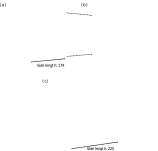
\includegraphics[keepaspectration, width=0.99\linewidth ]{\FitzHughNagumoFigures/BoxSizeInvariance/BoxSizeInvariance.pdf}
    \caption{\label{fig:TypicalSimulation} (a) A snapshot of a typical simulation, here of the $7_2$ knot $T=2420$ after initialisation, demonstrating the structure of the wavefield in a periodic simulation box. The level set $|{\bf B}|=0.4$ (red tube) marks the vortex filament, and contours of $ u = 1.6$ mark the location of propagating wavefronts (orange paired surfaces). The near quarter of the wavefronts are clipped to reveal their inner structure. The wavefronts have a complex topology at lengths comparable to that of the vortex, but away from it take the form of simple concentric shells. (b, c) Snapshots of the same $7_2$ knot evolution simulated in boxes of different sizes. (b) replicates (a), with a cross section through the $u$ wavefield shown (wavefronts in red). (c) shows the corresponding knotted vortex and wavefield from the larger box (dark grey simulation box corresponds to cross section shown). Differences in the wavefields are localised to the boundary of the smaller simulation box, ensuring we are indeed capturing bulk dynamics. As expected, the knot loci themselves are identical.}
\end{figure}
Stacking two-dimensional spiral vortices one obtains the simplest example of a vortex filament, one with a straight geometry from which emanates a quasi-two-dimensional `scroll wave'~\citep{Winfree1983}. More generally, the vortex filament is a tubular structure with arbitrary geometry, normal cross sections of which resemble spiral vortices whose phase is allowed to vary longitudinally. (In fact even this picture is an idealisation; waves emanating from other sections of the filament can disrupt this local spiral wave structure.) Various operational definitions to extract a one-dimensional curve from this tubular structure have been proposed~\citep{Winfree1990,Henze1993,Dowle1997}. Here we follow Refs.~\citep{Sutcliffe2003,Maucher2016,Maucher2017,Maucher2018,Maucher2019} and first compute the intermediate quantity
\begin{equation}
\label{eq:ucrossv}
\mathbf{B} = \nabla u \times \nabla v.
\end{equation}
$|\mathbf{B}|$ measures the deviation of $u$ and $v$ contours from colinearity --- it is zero for a planar wave, and only attains substantial nonzero value along the vortex filament. Contours of $|\mathbf{B}|$ thus take the form of tubes. For example, figure~\ref{fig:TypicalSimulation} tracks the vortex filament by showing the level set $|{\bf B}| = 0.4$ in red. To extract a one-dimensional curve from such a tube, we first note that $\bf B$ orients the tube. Stepping along the tube in the direction given by this orientation, we connect maximal values of $|\mathbf{B}|$ in cross sections taken through it, resampling if necessary to give equidistant steps; a similar extraction procedure is detailed in Ref.~\citep{Winfree1990}. This raw curve is then smoothed to remove modes of frequencies comparable to $\lambda$, giving a smoothed curve from which we may compute curvatures and torsions via finite difference. (The choice of lengthscale for filtering is motivated by the observation that the most highly curved stable filament observed, a stable round unknot~\citep{Courtemanche1990}, has a circumference comparable to $\lambda$.) Typically we will use the term `filament' to emphasise the one-dimensional curve defined above, and `vortex' when we wish to discuss the full tubular stack of spiral waves surrounding this curve. This definition (and indeed other `instantaneous' definitions~\citep{Dowle1997}) gives rise to small amplitude oscillations in the geometry of the filament at period $\sim T_0$ which carry through to derived quantities such as knot length. We shall examine the spectrum of these oscillations in detail in \S\ref{sec:StableKnots}, but in subsequent plots showing length evolution we filter them out for clarity. 

As discussed above, vortex phase varies along the filament, framing our one-dimensional curve, and the twist of this framing may in principle affect both filament motion and vortex rotation period. We track it by computing $\frac{\nabla u}{|\nabla u|}$ along the filament and then smoothing as above. 

\subsection{Initialising a knotted vortex field}
\label{subsec:WavefieldInitialisation}

To initialise an arbitrary knotted vortex for simulation we adopt the basic strategy of Refs.~\citep{Sutcliffe2003,Maucher2016} in which a phase field $\phi( {\bf x}) \in \mathbb{S}^1$, ${\bf x} \in \mathbb{R}^3\setminus K$, is constructed which contains a phase singularity with the geometry of some desired vortex knot $K$. Thereafter, the winding of $\phi$ around the specified knotted phase singularity is translated into the winding of $(u,v)$ around the excitation-recovery loop of the FitzHugh-Nagumo model as one encircles the vortex filament via the map $ (u,v) = (2 \cos \phi - 0.4, \sin \phi - 0.4)$.

To construct a phase field $\phi$ containing a singularity along a given curve $K$, we first compute the solid angle function $\omega$ about $K$ using \eqref{eq:OurSolidAngle1} from \S\ref{sec:CurveIsotopies}~\citep{Binysh2018} 
\begin{equation}
    \omega({\bf x}) = \int_{K} \frac{{\bf n}_\infty \times {\bf n} \cdot \mathrm{d}{\bf n}}{1 + {\bf n} \cdot {\bf n}_\infty} \quad \mathrm{mod}\;4\pi,
    \label{eq:SolidAngle}
\end{equation}
where for ${\bf y} \in K$, ${\bf n} := \frac{{\bf y} - {\bf x}}{|{\bf y}-\bf{x}|}$ is the projection of $K$ onto a unit sphere centred on $\bf x$ and ${\bf n}_\infty$ is an arbitrary unit vector. For a discussion of this integral and its numerical properties, including its singular behaviour about points ${\bf x}$ such that ${\bf n} \cdot {\bf n}_\infty = -1$, see~\S\ref{sec:NumericalImplementation} \citep{Binysh2018}. 
    

The solid angle contains the necessary phase singularity along $K$, and for the simulations discussed in this chapter we use it for initialisation directly by setting $\phi = \omega/2$. We briefly note, however, that the structure of $\omega$ about $K$ does not mirror that of a typical $(u,v)$ wavefield, which consists of a series of approximately equispaced wavefronts radiating outwards from the vortex filament (figure \ref{fig:TypicalSimulation}). Further, this methodology does not give control over the initial twist distribution along the filament, which is set by the intersection of the level set $\omega=0$ with $K$, the solid angle framing of $K$ discussed in~\S\ref{sec:LocalStructure}~\citep{Binysh2018}. We may control both of these features by modifying $\phi$ as
    
\begin{equation}
\phi({\bf x}) = k_0 d({\bf x}) + \frac{1}{2} \omega({\bf x}), 
\label{eq:WavefieldInitialisation}
\end{equation}
where $k_0 := 2\pi / \lambda_0$ is the spiral wavenumber and $d({\bf x}):= \mathrm{min}_{{\bf y} \in K} |{\bf y}- {\bf x}|$ is the minimal distance from ${\bf x}$ to $K$. $k_0 d({\bf x})$ increases linearly with distance from the curve, giving a periodic modulation of $\phi$ and hence $(u,v)$ with distance. As an example, figure~\ref{fig:WavefieldInitialisation}(a) shows the wavefield generated using~\eqref{eq:WavefieldInitialisation} when $K$ is a trefoil knot. The intersection of the level set $\phi=0$ with $K$, and hence the initial twist distribution, may be controlled by including an offset in the definition of $d({\bf x})$ which varies along $K$. An example of such a modulation, and how it alters the wavefield, is shown in figure~\ref{fig:WavefieldInitialisation}(b). Given, for example, the importance of twist distribution on both rotation frequency and the sproing instability as discussed above (and further explored in this chapter), such control is desirable for future work.

Initialisation geometries for the knots considered here were constructed from those found in \emph{KnotPlot}~\citep{KnotPlot}, which in turn are based on Rolfsen's knot table. In the absence of existing work on high crossing number knots in the FitzHugh-Nagumo model, there is no compelling reason to choose one set of initialisation geometries over another; for example, an alternative choice would be to use configurations of ideal ropelength~\citep{Cantarella2011,Kleckner2016,Maucher2017}. We use Rolfsen's configurations as, with the exception of the torus knots (whose evolutions we will compare to existing results~\citep{Maucher2017}) the geometries do not possess any symmetries. If strands of the knot are initialised closer to one another than the vortex radius $\lambda_0 /2\pi$, reconnections may occur in the first $\Delta T \approx T_0$ of simulation, before the wavefield about the knot is established~\citep{Maucher2016}. To ensure this does not occur, given an initialisation geometry $K$ we scale isotropically such that the longest side of $K$'s bounding box occupies $80\%$ of the simulation box size. As the simulation box is $O(50)$ times the size of the vortex radius, this ensures reconnections do not occur during initialisation. 

\begin{figure}[htbp]
\centering
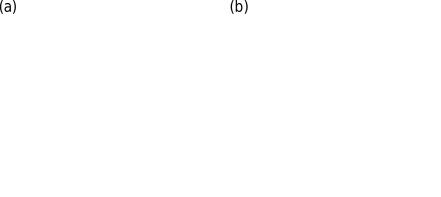
\includegraphics[keepaspectration, width=0.85\linewidth ]{\FitzHughNagumoFigures/WavefieldInitialisation/WavefieldInitialisation}
\caption{Wavefield initialisation about a trefoil knot vortex filament (red curve) using~\eqref{eq:WavefieldInitialisation}, with the level set $\phi = 0 $ shown in orange. The near half of the level set is clipped to reveal its inner structure. In (a) the definition of $d({\bf x})$ in~\eqref{eq:WavefieldInitialisation} is simply minimal distance to the filament. In (b) it is modified by a threefold symmetric sinusoid along the trefoil, effectively adjusting the solid angle framing and local twist rate of the vortex filament.}
\label{fig:WavefieldInitialisation}
\end{figure}


\section{\label{sec:UnstableKnots}Unstable Knots}

\begin{figure}[htbp]
\centering
    \includegraphics[width=0.99\linewidth]{\FitzHughNagumoFigures/UnstableKnotsLength/UnstableKnotsLength_annotated.pdf}
    \caption{ Length evolution of knotted vortices up to and including crossing number $N=8$, with reconnection events indicated by curves which terminate early with a circular marker. Knots included in the legend are further discussed in the text. Note the difference in scale between the first and subsequent panels. (a) $N\leq5$. (b) $N=6$ (dotted lines) and $N=7$ (solid lines). (c) $N=8$. The unknot ($0_1$), trefoil ($3_1$) and figure eight ($4_1$) settle to a stable length and fixed geometry (see section \ref{sec:StableKnots}). However, beyond this, generic behaviour is an initial period of contraction, followed by length increase over longer timescales. Insets show the geometries resulting from the destabilisation of the initially symmetric $5_1$ and $7_1$ torus knots.} 
\label{fig:UnstableKnotsLength}
\end{figure}

\begin{figure}[htbp]
\centering
    \includegraphics[width=0.99\linewidth]{\FitzHughNagumoFigures/Reconnections/ReconnectionsFigure.pdf}
    \caption{Reconnection of the $7_2$ knot at $T=2423$ (orange curve, then orange and green curves after reconnection event) shown in $\Delta T = 2$ increments. A pair of anti-parallel strands (circled in black) interact, generating a wavefield locally similar to that of the stable unknot; shown is the value of $u$ in a cross section through the knot, with high $u$ value coloured red. The wavefield from the remainder of the knotted filament, shown entering the circled region at $T=2417$, impinges upon these strands causing them to destabilise and reconnect. Note that the wavefield at $T=2420$ is also shown in figure~\ref{fig:TypicalSimulation}.}
\label{fig:Reconnections}
\end{figure}

Fascinating recent numerical experiments on the evolution of unknots initialised in complex geometries showed that the FitzHugh-Nagumo dynamics is capable of simplifying an initially tangled unknot to a unique circular curve, without strand crossings~\citep{Maucher2016}. These intriguing examples, coupled with two further instances of simplification in the case of the trefoil~\citep{Sutcliffe2003}, as well as some indirect evidence of the same behaviour for the Hopf link~\citep{Maucher2019} (and a series of preliminary results on various links in Ref.~\citep{Henze1993}), naturally invite the speculation that such simplification is generic to any knot. To investigate the dynamics of a generic knotted filament, and establish whether this is indeed the case, in figure~\ref{fig:UnstableKnotsLength} we show a survey of the length evolution of all knots up to and including crossing number $N=8$, with particular curves that we discuss further highlighted in the legend. Excluding chiral variants, there are thirty-six such knots. 

Initial behaviour across all knots is contraction; this behaviour is purely a result of curve geometry, reflecting an effective positive line tension for filaments well separated from any interactions~\citep{Biktashev1994}. Our curves are initialised with their strands separated by several vortex radii. Over the first few vortex rotation periods the wavefield establishes itself around the vortex filament (over such a timescale the filament may be considered stationary) with the resulting collision interface disjoint from the filament itself. Thereafter each segment of the filament initially moves effectively in isolation from its neighbours. 

Over longer timescales, however, we find that this initial contraction does not generically lead filaments to settle to a canonical form or a fixed length, and further that their topology is not always preserved. We observe reconnection events in eight of the thirty-six cases, indicated by those curves terminating in circular markers in figure~\ref{fig:UnstableKnotsLength}. The first of these occurs at $N=7$, with four of the seven $N=7$ knots and four of the twenty-one $N=8$ knots exhibiting reconnections.

Figure~\ref{fig:Reconnections} shows the reconnection event in the $7_2$ knot occurring at $T=2423$ in $\Delta T=2$ increments, with the region where the reconnection occurs circled in black. A pair of neighbouring anti-parallel segments are directly impacted by waves emanating from the rest of the knotted filament, causing them to destabilise and reconnect --- the same wave slapping mechanism responsible for the annihilation of a small unknot by a larger one observed in Ref.~\citep{Maucher2018}. In cross section, the wavefield generated by the anti-parallel segments (that section of the wavefield ending at the circled anti-parallel segments in the $T=2417$ panel of figure 4) locally resembles that of a stable unknot, or indeed of a pair of oppositely signed two-dimensional vortices~\citep{Courtemanche1990}. However this stable structure is additionally impinged upon by the wavefield of the rest of the knot (shown entering the circled region at $T=2417$). It has previously been noted that the rotation period of a stable unknot is 14\% greater than $T_0$~\citep{Maucher2018}, and as such the stable unknot is vulnerable to wave-slapping induced annihilation, as it cannot `fend off' a wavetrain of period $T_0$. This same argument applies to the anti-parallel segments discussed here, but the resulting topological change is reconnection. In addition to the similarity of the wavefields between the coaxial unknots of Ref.~\citep{Maucher2018} and the situation discussed here, the relative filament motion is also the same; in both cases, the perturbed filaments are drifting away from the impinging wavefield when topological change occurs. This geometric detail is important, as the velocity of a stable unknot ($0.3$~\citep{Maucher2018}) is a substantial fraction of the wavespeed in the medium ($1.9$) and as such Doppler shift may compensate for reduced unknot frequency. For the geometry here, however, the two effects can only compound one another. 

Topology changes previously reported in the literature have primarily occurred at simulation boundaries~\citep{Maucher2017, Maucher2019}, and one might be concerned that this reconnection is also an artefact of a finite simulation box. The snapshot of a $7_2$ simulation at $T=2420$ shown in figure~\ref{fig:TypicalSimulation} was taken from the same data shown in figures~\ref{fig:UnstableKnotsLength}, \ref{fig:Reconnections}, and was chosen specifically to emphasise that this is not the case. Enlarging the simulation box to side length $225$ as shown in figure~\ref{fig:TypicalSimulation} yields identical knot evolution, including the reconnection event.

Although we have focused the above discussion on the reconnection in the $7_2$ knot, analogous findings hold for the other cases. A detailed understanding of the wavefield evolution leading to such reconnections, and why they are seen here only for $N>5$, is lacking (we shall see examples of similar wavefield induced effects for small $N$ in \S \ref{sec:StableKnots}), but as $N$ increases one generically expects a more complex wavefield surrounding the knot as strands become closely packed over one another. As such, we lose the ability to picture segments of the knot as isolated, or even as interacting solely with a unique `nearest neighbour' region, but instead must think of them analogously to the vortex ring buffeted by external waves.

Even in the absence of reconnections, we only see stable states for the unknot, trefoil and figure eight knots; we shall discuss the robustness and detailed geometry of these states in \S \ref{sec:StableKnots}. For $N>4$ knots do not simplify. After the initial relatively rapid contraction, we generically see expansion over a much longer timescale of order several hundred vortex rotation periods followed by periods of irregular evolution including possible further expansion. Although the broad trend is to faster expansion at higher crossing number, the variability of behaviour between knots of the same crossing number suggests that initialisation geometry is just as important in determining long time evolution. In particular, we note the discrepancy between the behaviour of a typical knot with no initial symmetry and a torus knot initialised with high symmetry. Although a typical knot shows length increase by time $T\approx2000$, for the $5_1$ knot shown in figure~\ref{fig:UnstableKnotsLength} this increase is only visible by $T\approx4000$, and is not evident for the $7_1$ even by $T\approx6000$, although the inset curve geometries demonstrate the knot has indeed destabilised (that such destabilisation occurs, but only after long time simulations, clearly demonstrates the necessity of simulating for many hundreds of rotation periods before drawing conclusions about the dynamics of this system). In the next section, we shall investigate the mechanisms of both the dramatic length increases seen in a generic knot, and of the deviation of the torus knots away from initialisations of high symmetry. 
\begin{figure*}[htbp]
\centering
    \includegraphics[width=\textwidth]{\FitzHughNagumoFigures/63evolution/6_3}
\end{figure*}
\subsection{The mechanism of vortex knot length increase}
\label{subsec:Mechanism}
\begin{figure*}[hbtp]
    \caption{(overpage) Dynamics of the $6_3$ knot. (a) From $T=0$ to $T=2000$ the knot contracts and flattens, behaviour caused by the intrinsic curvature driven dynamics of an isolated filament mimicking a line tension. From $T=2000$ onwards length increases, with a single arm of the knot rapidly expanding outwards from an otherwise tightly packed core. (b) Comparison of the length evolution of the fully interacting $6_3$ vortex filament at $T=2000$ (green) to a copy encased in a `glass tube' of radius 10 (blue) or 15 (orange). With long-ranged interactions removed, the knot does not expand, but rather settles to a length of $\sim 400$ -- $600$. (c) Initial divergence in geometries between the interacting $6_3$ knot (green curve) and the radius $10$ tubed one (blue curve). Divergence does not occur globally, but is localised to two distinct expanding segments outside the lengthscale defined by the tube. (d) Distribution of filament twist during knot expansion. The expanding arm of the knot has twist values well below the $0.024$ rotations per space unit threshold for the sproing instability, and is less highly twisted than other, non-expanding, segments of the knot, ruling out this instability as the cause of length increase.}
\label{fig:63evolution} 
\end{figure*}
Exploring the knot geometries corresponding to the generic length increases seen in figure~\ref{fig:UnstableKnotsLength} one finds that, despite the variety of behaviour across knots, the increase occurs via a common mechanism in which isolated strands of the knot rapidly expand outwards from a tightly packed core region forming the rest of the knot. We illustrate this behaviour for the example of the $6_3$ knot in figure~\ref{fig:63evolution}(a). The same wave slapping mechanism driving reconnection events has also been proposed as a non-local mechanism for persistent knot length increase; in this context when the collision interface intersects a section of the knot, wave-vortex interactions drive that section outwards~\citep{WinfreeChapter,Sutcliffe2003}. The interaction does not have an intrinsic lengthscale, as waves in the medium do not decay. Instead, its range depends upon the geometry of the knot and the accompanying collision interface. For the $6_3$ knot shown in figure~\ref{fig:63evolution} one may verify that this surface intersects the expanding arm, suggesting that wave slapping may be at play. 

Given the potential importance of this mechanism, we would like to establish that it is really driving knot expansion, rather than simply being correlated with it. To do so, we investigate the effects of abruptly removing long-ranged interactions entirely, by numerically encasing the filament in a `glass tube' of moderate radius which moves with the filament and fuses when two knot segments approach one another~\citep{Winfree1983b}. With this construction short-range inter-filament repulsion, and geometry (including twist) mediated filament motion are preserved but long-ranged interactions are cut out. Using it, we may compare the evolution of a filament both with and without long-range interactions. A suitable radius for the tube is suggested by previous estimates of vortex radius in the literature, as well as the naive estimate $\lambda_0/2 \pi \approx 3.4$: Ref.~\citep{Courtemanche1990} directly measures a stable vortex ring radius of $4.8$, suggesting a vortex radius of $\sim~5$, and Ref.~\citep{Maucher2017} estimates a radius of $5.9$ by matching ideal ropelength~\citep{Cantarella2011} and measured trefoil lengths. To implement this construction numerically we simulate only within a tube of lattice points about the filament (the filament itself being constructed as in \S\ref{sec:Methodology}). In principle the details of the boundary conditions between the vortex and tube must be considered, however we have found that provided we use a tube radius above the vortex size estimates above, such details do not alter the geometry driven motion of the vortex, a reflection of its localised nature. This observation allows us to sidestep a sophisticated finite-element scheme (the spectral method discussed in \S~\ref{subsec:Simulation} only being valid for a periodic box), and instead simply use a finite difference method, with $(u,v)$ values for points outside of the tube set to their fixed point values $(-1.03,-0.66)$. The tube must move with the vortex, however we note that this need only happen on the (slow) timescale of vortex motion; we may allow motion in a fixed tube for a time $O(T_0)$, after which the tube is recentred around the vortex. The points brought into the tube at its boundary during this procedure are again set to fixed point $(u,v)$ values. In practice we typically use a conservative tube radius of $\sim 10$ with gridspacing $\Delta x = 0.5$ and timestep $\Delta t = 0.01$, with a finite difference scheme in which the Laplacian is computed using a seven point stencil and both reaction and diffusion terms are evolved using fourth order Runge-Kutta timestepping. The timestep above is chosen as it gives results identical to those of the spectral method using $\Delta t = 0.1$ when measuring the two-dimensional spiral vortex period. 

Figure~\ref{fig:63evolution}(b) contrasts the length evolution of the fully interacting $6_3$ knot with a copy of it encased in the tube, with initial conditions for both taken at $T=2500$, midway through knot expansion. Upon removing long-ranged interactions we no longer see a dramatic increase in knot length. Instead, the length of the tubed knot stabilises at $\sim 400- 600$. The details of this stabilisation vary depending on the radius of the tube, but the final lengths obtained are approximately the same across radii. Using the core size estimate of Ref.~\citep{Maucher2017}, the ideal ropelength of the $6_3$ knot is $340$~\citep{Cantarella2011}, and thus the tubed knot is relatively tightly packed. Over longer timescales ($\Delta T=8000$ shown for the radius $10$ tube of figure~\ref{fig:63evolution}(b)) the tubed $6_3$ does not reach a fixed geometry, but rather undergoes a compact tumbling motion, as the binormal component of filament motion causes segments of the knot to work over one another, though without further substantial length change. In figure~\ref{fig:63evolution}(c) we explore the initial divergence in geometry between the fully interacting and tubed knots. We see that it does not occur globally, but is localised to distinct expanding segments of the interacting $6_3$ which lie separate to the knot core region and are responsible for global length increase; these same segments are those which intersect the collision interface. Within the core region, segments of the filament are packed closer than the spatial cutoff we have defined, and there is no immediate divergence between the interacting and tubed knots. By contrast, removing long-range interactions allows distant segments of the tubed knot to evolve under their intrinsic dynamics, unaffected by wave-vortex interactions, and so shrink towards the core region. Thus a wave slapping mechanism accounts for global changes in knot length and also for the geometry of where they occur. 

In local geometric models of filament motion a mechanism by which filament length may stabilise or increase, despite an effective positive line tension, is via the `sproing' instability~\citep{WinfreeChapter} in which, above some critical local twist threshold, an initially straight filament expands into a helix --- for the FitzHugh-Nagumo model with the parameter values used here, Ref.~\citep{Henze1993} reports this threshold at 0.024 rotations per space unit for a straight filament. This instability has been proposed to account for the halting of links at lengths greater than hard core repulsion on the scale of the vortex radius would suggest~\citep{WinfreeChapter}, and for the destabilisation of symmetric torus knots~\citep{Maucher2017}. We may rule out sproing as a driver of the dramatic length increases seen in generic knots by noting that, as a local geometric mechanism, its effects were present in the tubed knot discussed above. For further confirmation, we may also examine the twist distribution along the fully interacting filament during knot expansion. Figure~\ref{fig:63evolution}(d) shows this distribution for the $6_3$ knot; we see that the expanding arm of the filament consistently has twist values well below the sproing threshold and, further, that other sections of the knot are more highly twisted, yet do not show the same length increase. In fact, twist values along the entirety of the knot are consistently below the sproing threshold, an observation also made for the early short time simulations of Refs.~\citep{Henze1993,WinfreeChapter}. 

Although not a driver of generic knot length increase, this last observation suggests that the sproing threshold may still have dynamical importance as a stabiliser against curvature induced length decrease, or play a role in the destabilisation of symmetric torus knots. In figure \ref{fig:TorusDestabilisation} we study the destabilisation of the $5_1$ torus knot, originally presented in figure \ref{fig:UnstableKnotsLength}, in more detail. Figure \ref{fig:TorusDestabilisation}(a) shows the evolution of a measure of the asymmetry of the knot, defined by taking the power spectrum of the knot's curvature as a function of arclength, and computing the fraction of the power in modes which do not respect the underlying symmetry (fivefold in this case). Alongside it we show the evolution of both the maximal twist, expressed as a fraction of the $0.024$ rotations per space unit sproing threshold discussed above, and the fraction of the arclength of the $5_1$ which attains a twist greater than $90\%$ of this threshold. We first note that the order of events is broadly consistent with sproing threshold playing a role in the dynamics. After an initial period in which the knot flattens and the twist remains roughly constant, maximal twist increases until it attains the sproing threshold, thereafter remaining constant; this threshold is attained as the length of the $5_1$ stabilises. However, it is several hundred rotation periods before we see the subsequent loss of symmetry. This timescale suggests that it is not the case that the knot hits the sproing threshold, and then destabilises; Ref.~\citep{Henze1993} notes that the timescale for sproinging to occur is typically only a few rotation periods. Furthermore the geometry of the destabilisation is inconsistent with sproing instability. In figure~\ref{fig:TorusDestabilisation}(b) we show the knot as it destabilises, coloured by twist. We fail to see helical sproinging along the highly twisted segments of the knot; instead the whole form collapses to a twofold symmetric shape. A similar deformation is seen in the $7_1$ (see inset of figure \ref{fig:UnstableKnotsLength}) and has been noted in early simulations of initially symmetric triply-linked rings~\citep{Henze1993}, where its cause was attributed to an interplay between the sproing threshold and inter-filament interactions. Overall, then, it appears the sproing threshold acts to halt knot shrinkage, but that subsequent destabilisation cannot be directly attributed to the sproing instability. 

\begin{figure}[htbp]
\centering
    \includegraphics[width=0.7\linewidth]{\FitzHughNagumoFigures/TorusDestabilisation/TorusDestabilisation.pdf}
    \caption{ The role of the sproing instability in the destabilisation of the $5_1$ torus knot. (a) shows the (normalised) length evolution of the $5_1$, alongside a measure of its asymmetry. Shown also is the maximum absolute twist along the knot as a fraction of the 0.024 rotations per space unit sproing threshold, and the fraction of arclength which attains 90\% of this threshold. The twist threshold is reached as knot length plateaus, but no sproinging instability is observed; instead the knot gradually destabilises over several hundred rotation periods. (b) shows the geometry of the knot destabilisation, coloured by twist. Rather than a helical instability developing in regions of high twist, the whole knot transitions to a twofold symmetric form.}
\label{fig:TorusDestabilisation}
\end{figure}

\section{\label{sec:StableKnots}Stable Knots}
\begin{figure}[htbp]
    \includegraphics[width=0.99\linewidth]{\FitzHughNagumoFigures/SecretKnots/SecretKnots.pdf}
    \caption{ Untangling dynamics of the (a) 18 unknots, (b) 17 trefoils and (c) 9 figure eight knots formed by performing single strand crossings on the higher crossing number knot geometries of \S \ref{sec:UnstableKnots}. (a) All unknots simplify to a unique round geometry without reconnection events. Length decrease is monotonic, however there is some variation; the geometry of one particularly slow decay is shown in the inset, displayed at times indicated by the solid markers. (b) All trefoil geometries simplify to a unique stable state, however there is greater variation across decays than for the unknots, with periods where knot length actively increases (boxed inset, circled markers). (c) Of the $9$ tangled figure eights simulated, $7$ settle rapidly to a stable state. However, over $T=20000$ one example fails to converge and another converges only after going through prolonged periods of length increase, contraction and irregular `tumbling' dynamics.} 
\label{fig:SecretFourOneLength}
\end{figure}

In \S \ref{sec:UnstableKnots} we showed that the speculation that a generic knotted vortex might simplify to a canonical form --- a speculation previously evidenced by promising `untangling' results for the unknot~\citep{Maucher2016} and a few further examples of simplification in low crossing number knots and links~\citep{Sutcliffe2003,Maucher2019} --- is not borne out for $N>4$. In the search for stable knots, recent numerical experiments found that knots and links could be stabilised through proximity to a no-flux boundary~\citep{Sutcliffe2003,Maucher2017}. Primarily the examples shown were for torus knots and links, although the figure eight knot and Borromean rings were also briefly given as non-torus examples. In contrast to the untangling of unknots, these boundary stabilised states of more complex vortices were not established to be `basins of attraction' for generic initial geometries, but rather were obtained from highly symmetric initial vortex line geometries. In \S \ref{sec:UnstableKnots} we also saw that in the case of torus knots more complex than the trefoil such states are not stable in our bulk simulations. By contrast, for the stability of the trefoil and figure eight knots we now show that a much stronger statement than has been made previously is true: in the bulk, a generic trefoil or figure eight simplifies to a canonical form, analogously to the unknot. The states are the same as those found in the survey of figure \ref{fig:UnstableKnotsLength} and also appear to be the same as those found near a reflecting boundary. In addition, we strengthen the results of Ref.~\citep{Maucher2016} and demonstrate them to be independent of a no-flux boundary by testing the bulk untangling dynamics of the unknot with a far greater variety of initial conditions than has been used previously.

All knots may be converted into the unknot by performing strand crossings. The minimal number of strand crossings needed to convert a knot into the unknot is called its unknotting number. Of the knots with $N\leq8$ there are $18$ with unknotting number $1$; that is, they can be converted to the unknot by a single strand crossing. By analogous single strand crossings one can also target the trefoil or figure eight knots: for $N\leq8$ there are $17$ that convert to the trefoil and $9$ to the figure eight under a single strand crossing. Beginning with the knot geometries of \S \ref{sec:UnstableKnots}, we use these crossings to provide an assortment of initial tangled geometries for unknots, trefoils, and figure eights, and study their evolution. Figure~\ref{fig:SecretFourOneLength}(a) summarises the results of these simulations for the tangled unknots. We find in all cases that the initially tangled vortex transforms to a unique stable ring and that the dynamics does not involve any reconnections. The typical dynamics is an approximately constant rate of length contraction, although this is not rigorous and there is some variation. In particular, in one example (obtained from the $8_{11}$ knot) there is a substantial period of pause where length decreases much more slowly than is seen on average; snapshots of the geometric evolution of this curve are shown as insets. 

Figures~\ref{fig:SecretFourOneLength}(b),(c) show results for the trefoil and figure eight knots. As with the unknot, for the trefoils we see simplification without reconnection to a unique steady state, although there are perhaps more examples showing periods where the length is not decreasing; one such is illustrated by the inset figures. However, for the figure eights the dynamics is rather more complicated; $7$ of the $9$ initialisations rapidly converge to a unique stable state, but $2$ show prolonged periods of length increase as well as of contraction, with one of them failing to converge over the times simulated. In the example highlighted in figure~\ref{fig:SecretFourOneLength}(c), we see that the initial period of expansion is due to a single arm of the knot rapidly expanding outwards from an otherwise tightly packed core, caused by the same wave slapping as described in \S\ref{sec:UnstableKnots}. This expansion continues for many hundreds of rotation periods and results in a total increase of several times the initial knot length. In addition, the subsequent period of contraction does not lead directly to a stable shape, but rather produces an extended period of `tumbling' dynamics in which the length fluctuates erratically before eventually settling to the final steady state. The total time that this dynamics plays out over greatly exceeds that of the typical unknot. 

These results bridge the gap between the simplification of the unknot discussed in Ref.~\citep{Maucher2016} and our own findings for high crossing number knots by showing that, although clearly neither the untangling dynamics nor the geometries giving rise to wave slapping instability are fully understood, the same mechanisms dominating high crossing number knot behaviour also play an important role in determining low crossing number behaviour; wave slapping can totally disrupt the appealing picture of a dynamics which monotonically decreases knot length even when a stable target state exists. The results also demonstrate the importance of initial conditions on long-term knot evolution; even given the existence of a stable state, the difference between a `good' and `bad' initial starting state may lead to an order of magnitude difference in the time taken to reach that stable state. 

Another notable example of the importance of initial conditions comes from the observation that the boundary stabilised trefoil knot actually exists in two distinct stable configurations~\citep{Maucher2017}. The first, which we denote the $3_{1,1}$, has the geometry that the tangled trefoils of figure \ref{fig:SecretFourOneLength} evolve to. The second, which we denote the $3_{1,2}$, is not reached by our tangled trefoils. This state was constructed in Ref.~\citep{Maucher2017} from an exactly twofold symmetric initial vortex filament, and preserves this symmetry in the final reported state. Although, as we have seen with torus knots, highly symmetric boundary stabilised states may not exist in the bulk, in our own simulations we have found the $3_{1,2}$ to be accessible in the bulk using an initial configuration with only approximate twofold symmetry, and have confirmed its stability up to $T=12000$. Thus, although this twofold symmetric $3_{1,2}$ indeed appears stable, the results of our tangled trefoil simulations suggest that it has a small basin of attraction. Taken together, the above results suggest that, although we have seen that the stability of higher crossing number knots is not the norm, stable geometries may nevertheless exist in the bulk, but that when hunting for them we should not use any carelessly chosen initial configuration, but ought to be more selective in which initial geometries we use. For hints as to what those geometries might be, we now investigate in detail the properties of the stable knots we have found thus far.

\subsection{Properties of stable knots}
\begin{figure}[hbtp]
    \includegraphics[width=0.95\textwidth]{\FitzHughNagumoFigures/StableKnots/StableKnotsFigure.pdf}
    \caption{Geometries, vortex framings and twist distributions of our stable knots. Vector fields along curves indicate vortex framings, and are shown at four successive times across a (approximate) vortex rotation period. Curvatures and torsions shown correspond to the $T=0$ panels (there is slight intra-period variation) with the zero of arclength fixed to maximal curvature values. With the exception of the $4_1$ knot for which there is no distinction, all knots shown are the `right handed' chiral variant --- they rotate in a right handed sense about their direction of motion (down the page). Dotted circle highlights a half turn of a helix in the figure eight geometry, which may be extended to several half turns to give the initialisation geometries for the stable Whitehead link and $6_2$ knot shown. }
\label{fig:StableKnots}
\end{figure}

Figure~\ref{fig:StableKnots} shows the geometries, curvature and torsions as a function of arclength, vortex framings and twist distributions of the stable $3_{1,1}$, $3_{1,2}$ and figure eight knots. The evolution of their vortex framings at four successive intervals over a (approximate) vortex rotation period are indicated by the vector fields along the curves. Curvatures and torsions shown correspond to the geometries in the far left, $T=0$ panels (as discussed in \S \ref{subsec:DefiningTracking} there is slight intra-period oscillation), with the arbitrary zero of arclength fixed to coincide with maximal curvature values. We first note the striking twofold symmetry of both the $3_{1,2}$ and the $4_1$ knots; this symmetry is not a remnant of initial conditions, but emerges from the underlying dynamics. By contrast, the $3_{1,1}$ lacks any threefold symmetry. This is especially notable given that this state was reached starting from an exactly threefold symmetric torus knot geometry in \S \ref{sec:UnstableKnots}. It appears that the boundary stabilised trefoil reported in Ref.~\citep{Maucher2017} also lacks threefold symmetry, although it is unclear why this loss of symmetry does not occur for boundary stabilised torus knots of higher crossing number. A second striking feature of these stable knots is the tight synchronisation of the evolution of their framings. The framings of closely separated segments of the filament mesh~\citep{Henze1993}, the wavetip emanating from one segment being consistently met by a wavetip emanating from a spatially neighbouring segment, resulting in travelling waves of tightly synchronised wave activity running the length of the knot in a periodic fashion. The pattern is evident in the $3_{1,2}$ and figure eight knots, but is also present in the $3_{1,1}$, most clearly when one focuses on one of its three relatively straight segments; the framing of the curved lobes is twisted such that it meets the rotation of the wavetip emanating from the straight segment. Again, this meshing is an emergent property of the stable knot. 
\begin{figure}[htbp]
\centering
    \includegraphics[width=0.65\linewidth]{\FitzHughNagumoFigures/Stable_Whitehead_6_2/Whitehead_6_2.pdf}
\caption{Length evolution of the Whitehead link and the $6_2$ knot with initialisation geometries made by extending the structure of the stable $4_1$ knot. Insets correspond to marked times.}
\label{fig:Whitehead_6_2}
\end{figure}

The similarity of the geometries and vortex framings of the $3_{1,2}$ and figure eight is suggestive of a recurrent structural motif. To investigate further we take the geometry of the the stable figure eight and use it as a starting point to construct new trial initialisation geometries. We do so in the simplest way possible --- as highlighted in the dotted circle around a section of the $T=0$ figure eight in figure \ref{fig:StableKnots}, the knot geometry contains a half-turn of a helix, which we may extend to an integer number of half-turns. Doing so gives a family of trial initialisation curves alternating between knots and two component links, the next two being the Whitehead link and the $6_2$ knot. Simulation reveals that such initialisation geometries evolve to apparently stable states. Figure \ref{fig:StableKnots} shows their detailed geometry, and in figure \ref{fig:Whitehead_6_2} we confirm their bulk stability up to $T=15000$. Both states share the twofold symmetry and tight synchronisation over a vortex rotation period found in the $3_{1,2}$ and figure eight knots, with especially close similarity in the geometry and twist distributions of the $4_1$, Whitehead link and $6_2$ knots. This similarity suggests that they arise as the start of a family of such stable knots which does not cleave along some existing sub-category of knots (for example torus knots) but rather arises specifically from the FitzHugh-Nagumo dynamics. As another demonstration of the importance of initial conditions, and a reminder that such states may have small basins of attraction, we note that the $6_2$ of \S \ref{sec:UnstableKnots} does not find this stable state over the times simulated.

In figure \ref{fig:KnotDynamics} we explore the dynamical properties of all stable knots found thus far. With the exception of the $3_{1,1}$, we find that each drifts along its axis of symmetry and rotates as a rigid body, with speeds and rotation rates summarised in figure \ref{fig:KnotDynamics}(a); these rates are computed by averaging the motion of the rigid body frame of the stable knot over $\Delta T = 2000$. An example of this motion is shown for the $6_2$ knot in figure \ref{fig:KnotDynamics}(b) (as can be seen in figure \ref{fig:Whitehead_6_2}, the Whitehead link and the $6_2$ knot have some long timescale periodic length modulation which corresponds to a slight oscillation in their velocity). The $3_{1,1}$ instead drifts in a helix as shown in figure~\ref{fig:KnotDynamics}(c), rotating about the helical axis as a rigid body, a reflection of its lack of threefold symmetry (a numerical fit to this helix~\citep{Enkhbayar2008} finds that it has radius $3.23$ and pitch $39.34$). The scale, and structure with knot size, of the drift velocities resembles that found for torus links in Ref.~\citep{Maucher2019}: within the family of knots discussed above, we see drift velocity decreasing with knot size. However, the complex geometries of the stable knots discussed here renders the explanation for this decrease given for torus knots (decreasing asymmetry between inner and outer parts of the torus as size increases) inapplicable. A reflection of this complexity is that, beyond consistency of scale, there is no clear accompanying pattern in the rotation rate data.

We briefly note that in the above discussion of vortex rotation sense, drift velocity and overall knot rotation sense we have not been careful to distinguish the possibly different behaviours of oriented or chiral variants from one another. All stable knots and links discussed above are isotopic to themselves under reversal of the orientation of any link component, however with the exception of the $4_1$ they are all chiral, and this chirality determines the rotation sense of the knot. In figures \ref{fig:StableKnots} and \ref{fig:KnotDynamics} we present variants rotating in a right handed sense about their drift velocity; left handed variants, with reversed twist distributions, also exist.

As discussed in \S \ref{sec:UnstableKnots}, Ref.~\citep{Maucher2018} reports an increase in the rotation period of a stable unknot by $14\%$. We investigate whether similar shifts exist for other stable knots by looking at the spectra of their high frequency length oscillations. Figure~\ref{fig:KnotDynamics}(d) shows the spectra of all stable knots as measured over $\Delta T = 4000$ after they reach their stable configurations, alongside the spectra of the first $T=1000$ of the unknot and $4_1$ data shown in figure~\ref{fig:UnstableKnotsLength}. We include this second set of data for calibration and methodology validation, as during this time we expect the data to give the spectrum of a noninteracting knot, which should approximately correspond to $f_0$. As expected, the length oscillations of the noninteracting data are consistent with the fundamental vortex rotation frequency of $f_0=0.0898$, and do not vary with knot topology --- before inter-vortex interactions occur the global structure of the filament does not dramatically affect vortex rotation period. In fact, as this data is taken during the contraction of both knots, the observation that it shows purely spectral broadening suggests a negligible role for curvature in possible shifts to rotation frequency. As with the noninteracting data, the stable knot spectra show single peaks, but their frequencies are shifted relative to the noninteracting case on a scale which exceeds our estimate of curvature induced corrections. For all nontrivial knots, this shift is to a higher frequency (lower period), and its size is approximately constant; we obtain a period of $T=0.97T_0$. By contrast, the unknot alone shows a substantial shift to lower frequencies (higher period); we find an unknot rotation period of $T=1.19T_0$, consistent with the results of Ref.~\citep{Maucher2018}. That the situation for nontrivial knots is a shift to lower period relative to an isolated filament is intriguing, and suggests itself as a potential origin of the motion of the collision interface leading to the wave slapping observed in \S \ref{sec:UnstableKnots}. One important complicating factor in this sort of analysis is Doppler shift. Although the period of the stable unknot is higher than $T_0$, its velocity is $0.3$, a substantial fraction of the wavespeed $(1.9)$ in the medium. Using the data presented here this gives a Doppler shifted period for a stationary observer ahead of the unknot of only $1\%$ greater than $T_0$; in other words, at least for the unknot, relative filament motion is extremely important in determining the stability of a situation. A similar calculation for an observer behind the $4_1$ gives a Doppler shifted period of $T=0.975T_0$, a far less substantial shift. We speculate that these two facts, firstly that stable structures generically appear to have periods shifted below $T_0$, and secondly that even when the shift is to a higher period in the case of the unknot (extrapolating unknot behaviour to that of generic anti-parallel strands) this increase is compensated for in a directional manner by Doppler shift, give an intrinsically unstable dynamics in which the formation of any interacting structure hinders further formation via wave slapping.

\begin{figure}[htbp]
    \includegraphics[width=0.99\textwidth]{\FitzHughNagumoFigures/KnotDynamics/KnotDynamicsFigure.pdf}
    \caption{Dynamics of stable knots. (a) A summary of drift speeds and rotation rates for all known stable knots. Note that the velocity given for the $3_{1,1}$ is that along its helical axis. (b) Drift and rotation of the $6_2$ knot. Shown are centres of mass taken at $T=100$ intervals (blue dots), and snapshots of the geometry at $T=3000$ intervals; between each snapshot the knot has rotated $\sim 20$ times. (c) The $3_{1,1}$ drifts along a helical path (fitted red curve), rotating about the helix axis as a rigid body. (d) Power spectra of high frequency oscillations in knot length data. Before inter-vortex interactions occur, the oscillation period is the same as ${f_0}$. All non-trivial stable knots show a similar shift to higher vortex rotation frequencies ($T=0.97T_0$), with the unknot alone showing a shift to lower frequencies ($T=1.19T_0$).}
\label{fig:KnotDynamics}
\end{figure}
\section{\label{sec:Discussion}Discussion}

We have presented a survey of the bulk dynamics of knotted vortices in the FitzHugh-Nagumo model covering prime knots up to crossing number $N=8$. Although the simplest knots --- the unknot, trefoil and figure eight --- possess stable states and exhibit a fascinating dynamics of untangling without reconnections, this is not repeated for any of the other knots in our survey. The general trend is an irregular dynamics, marked by sustained periods of length expansion of parts of the knot, the cause of which we have directly shown to be a long-range wave slapping interaction. In several cases, this wave slapping led to strand reconnections and topology change, phenomena which appear to be associated more with the geometry of the wavefield than the topology of the vortex. 

For those stable knots found in our initial survey, we have tested the effectiveness of the FitzHugh-Nagumo flow in untangling a wide variety of initial conditions. Although the dynamics successfully untangled all but one initial geometry over the time simulated, we saw that in the case of the figure eight knot this untangling was far from monotonic, and that the same wave slapping dominating high crossing number knot behaviour may also cause low crossing number knots to substantially increase in length before untangling. These results stand in contrast to those of Ref.~\citep{Maucher2016} and our own on the rapid untangling of unknots. We gave a detailed characterisation of the geometry and dynamics of all known stable vortices in the bulk, including the tight synchronisation of their associated wavefields, their motion through the medium and natural rotation periods, and shifts in the spectra of their high frequency length oscillations. In addition to the already known trefoil and figure eight knots, we found stable forms for the Whitehead link and $6_2$ knot, both of which appear to come from the same `family' of knots as the figure eight. While in the former case, the basin of attraction appears to be large, the same cannot be said for the latter, at least for the timescales of the simulations we have run. 

Throughout this chapter, we have emphasised the importance of the collision interface on understanding long timescale vortex dynamics. Although we have seen many examples of its importance, an understanding of its own dynamics is currently qualitative at best. As a first step towards rectifying this, it would be interesting to directly study the evolution of local rotation rate along a vortex to fully disentangle the possible effects of curvature, twist and interactions. Turning from general dynamical questions to the details of stable states, beyond noting close similarities between those found we have not proposed principles by which their geometry and behaviour may be understood. A detailed description appears challenging, but the observed wavefield synchronisation, and similarities in the size of spectral shifts, of \S\ref{sec:StableKnots} offers a global organising principle from which one might try to predict geometries. When discussing stability we have contrasted our own results in the bulk with those on torus knots and links that have been found near no-flux boundaries~\citep{Maucher2017,Maucher2019}, detailing where results overlap (the stability of the trefoil and figure eight) and where they diverge. Although we have seen that boundary stabilisation is more complex than simply a suppression of the sproing instability, its exact nature remains unclear, and deserves further study. 

The features of the FitzHugh-Nagumo model at the parameter values studied here which are conducive to the formation of stable knots --- short-range inter-vortex repulsion, a contractile filament law of motion --- are offset by other undesirable features, primarily wave slapping. Parameter choices were originally made in Ref.~\citep{Henze1993} on the basis that such values gave two-dimensional vortices with desirable properties and three-dimensional simulations were computationally feasible. It would be interesting to revisit these choices armed with new criteria for a desirable set of parameters. For example, we might search for parameters (or indeed models) such that rotation frequency is seen to decrease with twist and interactions. A related question is to explore whether wave slapping interactions have any role in enhancing untangling as well as hindering it --- in other words, whether the untangling aspect of the dynamics can be captured in a local geometric model. Here the tubed knot of \S\ref{sec:UnstableKnots} offers some hints; in preliminary simulations of tubed versions of the tangled unknots of \S\ref{sec:StableKnots} we do not see substantial differences in the untangling times between tubed and untubed unknots. It may be the case that, although the full dynamics appear extremely difficult to capture with a local geometric model, such a model offers insight for the restricted case of unknot untangling. This is especially interesting given the apparent contrast between the untangling dynamics seen here and those utilised by line tension minimisation methods~\citep{Maucher2016}. 

Stable vortex rings have been realised experimentally and successfully described using existing theory~\citep{Steinbock2006, Azhand2014, Totz2015}. As such, although one expects the precise details of knot stability to be specific to the system studied, we believe that our exploration of the phenomena seen here --- the importance of wave slapping, bulk simplification of low crossing number knots, frequency shifts in stable knots --- is of direct experimental interest for a general excitable medium, outside of the details of the FitzHugh-Nagumo model. 


                            %% More chapters.
%!
%! There are a few variations of reference
%\begin{verbatim}\citet[chap. 2]{ballentine82}|
%\end{verbatim}
%for a textual one, as \citet[chap. 2]{ballentine82}.\\
% \\
%\begin{verbatim}\citep{abraham_etal}
% \end{verbatim}
% for a parenthetical citation \citep{abraham_etal},\\
%
% \begin{verbatim}\citep*{MTW}
% \end{verbatim}
% for a full list of authors use a * parenthetical citation \citep*{MTW},\\
% \\
%!!!!!!!!!!!!!!!

%  \appendix                            %% this will do the appendices
%  \chapter{Proof of Fred's theorem}
%  \input{app1.tex}
%  \chapter{listing of Fred's program}
%  \input{app2.tex}

\bibliographystyle{plainnat}

\bibliography{ThesisBibliography}            %% Start your bibliography here;
                                 %! with sample.bib as your bibliography file. You can
                               %% also use:
                %! \begin{thebibliography}
                %!    \bibitem{etc....
                %! \end{thebibliography}
                               %% to generate your bibliography.

%\begin{thesisauthorvita}             %% Write your vita here; it can be
%                                     %% anything in LaTeX2e par-mode.
%\end{thesisauthorvita}               %%

\end{document}                       %% Done.
